% Chapter 6

\chapter{The energy costs of commuting}
\label{Chapter6}
%The volatility of oil prices \cref{fig:oilprices}).
% This is the money shot chapter: maps of behaviour culminating in energy maps
% generated by msim
% Compare energy use estimates derived through msim vs agg methods (it allows
% estimates at a small geo. scale right???!!!)
\lhead{Chapter 6. \emph{The energy costs of commuting}} % Write in your own
The energy cost data presented in the previous chapter and the
individual and aggregate level datasets mentioned in
\cref{Chapter4} are combined in this chapter to produce estimates of
energy costs at national (\cref{snational}), regional (\cref{sregional}) and
individual (\cref{sindvar}) levels. The international applicability of the
methods is tested the energy use of commuting in \cref{sinternational}, which
compares the energy intensity of commuting in England and the Netherlands.
% Estimates of changes in the energy costs of work travel over time
% are presented in \cref{stime}.
% 
% After presenting these estimates, attention is directed towards
% factors accounting for the variability observed at all levels.
% \Cref{sexplanation}, explores possible causes of energy intensive
% commuter patterns with reference to the literature, the energy use estimates
% present in this chapter and 
% additional data sources. The aim here is to move beyond description and
% towards explanation, to
% % so \cref{sexplanation} sets !!! re-add
% set out the scene for policy implications:
% it is the \emph{understanding} of an issue that allows it to be tackled
% successfully, rather than mere knowledge of its existence
% (see \citealp{Berners-Lee2013}).
In the final section, we return to consider the complexity of the transport
system discussed in the previous chapter and how this impacts on the
confidence we can have in the energy use estimates.


% \section{Commuting behaviour}
% Although available transport technologies and infrastructure affect the energy
% use of travel to work patterns over space and time, as presented in
% \cref{Chapter5}, it is behaviour that determines how much energy using devices
% are used. This section therefore analyses the aggregate level transport to work
% data, to guide the subsequent analysis of energy costs.

\section{Commuter energy use at the national level} \label{snational}
Based on the data and discussion of it presented up until now, we are
well-placed to perform a preliminary estimate of energy use at the aggregate level.
This approach, starting simple to understand the fundamentals and most important
factors influencing the system before later adding details, follows the
recommendation of \citet{batty1976urban}.

Having considered the limitations of the data, and weighed up the
pros additional of complexity with the advantages of simplicity, it was decided to
primarily calculate $ET$ at the aggregate level,
as a function of only two parameters: mode and distance travelled.
(These are the cross-tabulated categorical variables provided as geographically
aggregated count data at administrative levels down to ST Wards ---
see \cref{t:agdata}). This can be expressed for any particular area as
\begin{equation}
 ET = \sum_m \sum_d{2dR_{(d,m)} \times E_m}
 \label{eqet1}
\end{equation}
where ET is the total work-day energy costs for all commuter trips that happen
in that area, d and m are distance and mode categories, dR is the mean average
route distance inferred from the the mode-distance combination and E an
estimate of the
energy cost per unit distance (direct or indirect), presented for each mode
in \cref{tfinale}.

An alternative way to express this would be based on commuter flow data.
If we know the approximate origins (i) and destinations (j) of every commuter
trip, this can be expressed in a different way:
\begin{equation}
 Et_i = \sum_j \sum_m {n_{(i,j)} \times 2Q \times dE_{(i,j)} \times Ef_m}
 \label{eqet2}
\end{equation}
where $Q$ is the circuity factor which translates the Euclidean distance between
two places into an approximation of the network distance, defined by \cref{eq:circ}.
Summing Et for all the origin areas in the region of interest would provide
an overall estimate of energy costs.

Clearly, neither \cref{eqet1} nor \cref{eqet2}
tell the entire story, as they omit frequency of travel: how many days
per week people travel to work (this is covered in \cref{sfreq}).
They also omit a number of other complicating factors that are discussed in
the previous chapter.  However, they are enough to begin with, to create maps
that capture the spatial variability of energy costs of commuting at
a coarse geographical resolution.
The approach summarised by \cref{eqet1} is used, because the input data
is much simpler, smaller and easier to manage. (\Cref{eqet2} could be used
to verify the estimates.)

The input variable into \cref{eqet1} that has not yet been quantified is
dR. Route distance by mode and distance band
is needed to account for the fact that Census data on distance is presented in
categories (with breaks at 2, 5, 10, 20, 30, 40 and 60 km), whereas distance
itself is continuous. The simplest way around this problem would be to
assume that route distance sits in the centre of the bins (i.e.~1, 3.5, 7.5, ...
km). However, this would be a very gross simplification because the route distance
is certain to be greater than the Euclidean distances calculated from
home-work postcode pairs. Also, because each mode has a different
distance-frequency distribution,
% !!! figure???
it is safe to say that the average route distance will also vary depending
on the mode of travel.\footnote{One would, for example,
expect people who walk 2 to 5
km in Euclidean distance to travel on average less far than those who drive
between 2 to 5 km, as `impedance' of walking rises rapidly after the first
kilometre whereas the additional personal effort of driving
an extra kilometre or two is much lower
\citep{Iacono2010}, discussed in \cref{Chapter2}.
}
To take this into account, distance data from Understanding Society was used.
% !!! major *** should have used NTS --- do after = priority!
First, the values were converted into estimates of Euclidean distance and
split into the Census bands. Next, these were re-converted into the original
route distances, and the average was taken for each distance band/mode
combination. The results, which are presented in \cref{tdboxes} and visualised in 
\cref{fdboxes} and \cref{fdboxes2} for motorised and non-motorised modes,
provide strong evidence of inter-mode variation in distance travelled within
the same distance band. However, these results are problematic due to the
low quality of the input data (n = 5,000 but less than 5 individuals
were present for unusual
categories such as people walking more than 5 km to work) and were not entirely
as expected. The anomalies are summarised as follows:
\begin{itemize}
 \item Bus journeys appear to be longer than the equivalent journeys by train,
 which was expected to be associated with the longest trips (although train
 journeys are in second place).
 \item The average bicycle trip was expected to be longer than walking trips
 in all cases. This did apply in the 0-2 and 2-5 km categories, but after that
 the trend reversed. This can be explained by sample size: a few unusual people
 walk far to work, whereas cyclists, as expected, tend to cluster around the lower
 ends of the 5-10 and and 10-20 km bins.
 \item The `inverse U' shape of the bottom graphs in both cases were unexpected.
 This could be explained by the tendency of people to round to 10: the
 average distance travelled in the 30-40 km bin was the closest to the upper
 bound in all cases, perhaps a result of people rounding to 25 miles for many
 trip distances in the 20s (just under 40 km in Euclidean distance)
\end{itemize}
It would be desirable to corroborate these findings with other individual level
data on travel to work. For the purposes of assessing the relative energy
costs of commuting in different areas, however, these estimates suffice:
the concepts and code behind the estimates would produce slightly different
values given different input data, but, at present, this is not our concern.
Our concern is that with evidence-based estimates of $dR_{(d,m)}$ in place,
we can proceed to estimate the relative energy costs of commuting in different
places. 

\begin{table}[htbp]
\caption[Average distance travelled by mode and distance band]
{Average distance travelled by mode and distance band (km),
from USd data.}\label{tdboxes}
\begin{center}
\begin{tabular}{lrrrrrrrr}
\toprule
Upper limit & 2.0 & 5.0 & 10.0 & 20.0 & 30.0 & 40.0 & 60.0 & 250.0 \\ \midrule
card & 1.6 & 3.9 & 7.9 & 15.0 & 26.0 & 35.8 & 50.3 & 102.6 \\
carp & 1.5 & 3.9 & 7.9 & 15.2 & 26.5 & 36.4 & 48.0 & 95.0 \\
moto & 1.4 & 4.1 & 7.0 & 15.2 & 23.5 & 36.0 & \multicolumn{1}{l}{NA} & \multicolumn{1}{l}{NA} \\
bus & 1.8 & 3.8 & 7.7 & 13.9 & 27.7 & 40.0 & 56.0 & 110.5 \\
train & 1.5 & 4.2 & 8.1 & 15.1 & 26.4 & 37.6 & 53.2 & 98.8 \\
metro & 1.7 & 4.0 & 8.1 & 14.7 & 25.8 & \multicolumn{1}{l}{NA} & \multicolumn{1}{l}{NA} & 65.0 \\
cycle & 1.5 & 3.9 & 7.5 & 11.5 & \multicolumn{1}{l}{NA} & \multicolumn{1}{l}{NA} & \multicolumn{1}{l}{NA} & \multicolumn{1}{l}{NA} \\
walk & 1.2 & 3.5 & 8.0 & 13.7 & 25.0 & \multicolumn{1}{l}{NA} & \multicolumn{1}{l}{NA} & \multicolumn{1}{l}{NA} \\
other & 1.0 & 4.3 & 7.6 & 13.5 & 27.8 & 37.5 & 42.0 & 130.0 \\
taxi & 1.7 & 3.0 & 9.0 & 12.0 & \multicolumn{1}{l}{NA} & \multicolumn{1}{l}{NA} & \multicolumn{1}{l}{NA} & \multicolumn{1}{l}{NA} \\
\bottomrule
\end{tabular}
\end{center}
\end{table}

\begin{figure}[htbp]
\begin{center}
    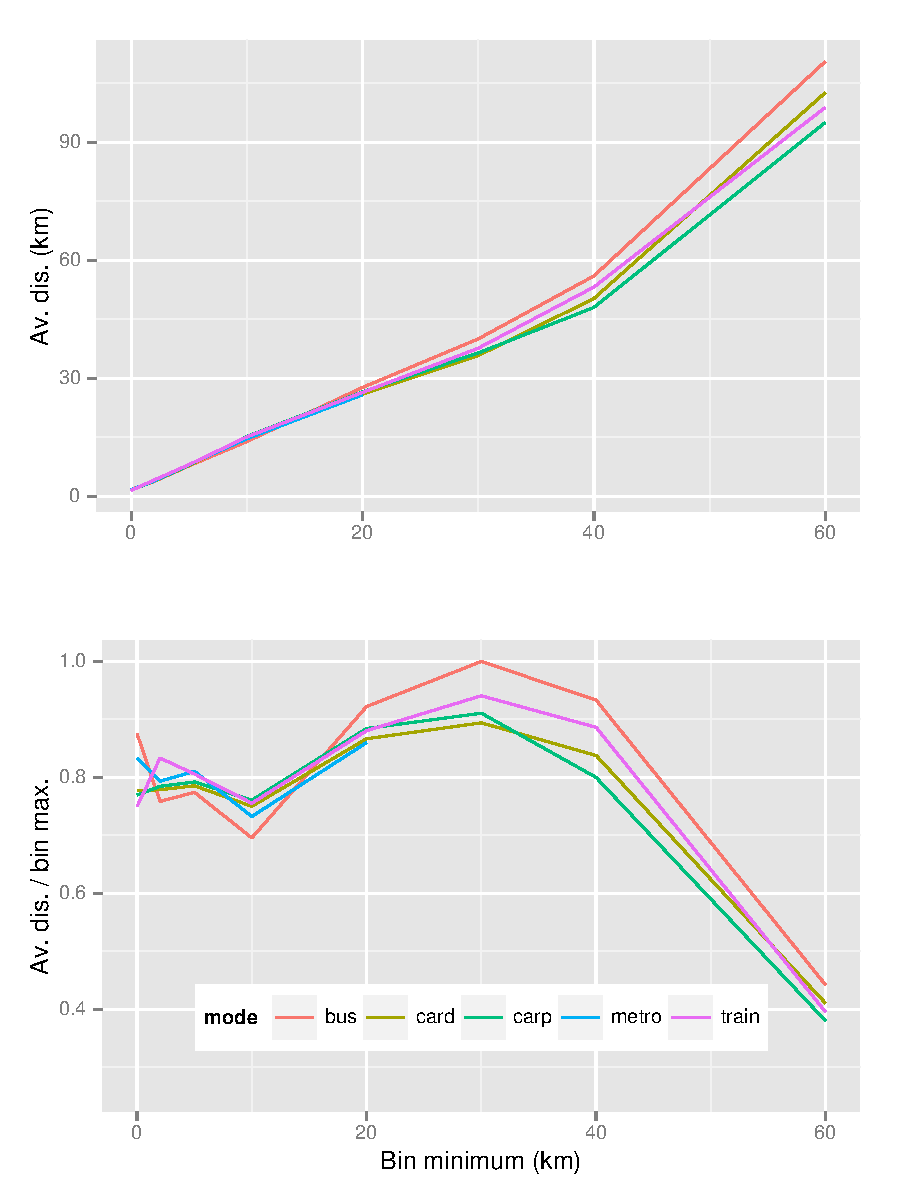
\includegraphics[width=9cm]{dboxes}\end{center}
  \caption[Distance bands and average distance travelled for motorised modes]
  {Distance bands and average distance travelled for motorised modes, expressed
  as the relationship between lower bound and average distance (top)
  and that between lower bound and the ratio of upper bound to average distance
  (below), from Understanding Society data.} %%% could update with NTS!!! should have used centre...
  \label{fdboxes}
\end{figure}

\begin{figure}[htbp]
\begin{center}
    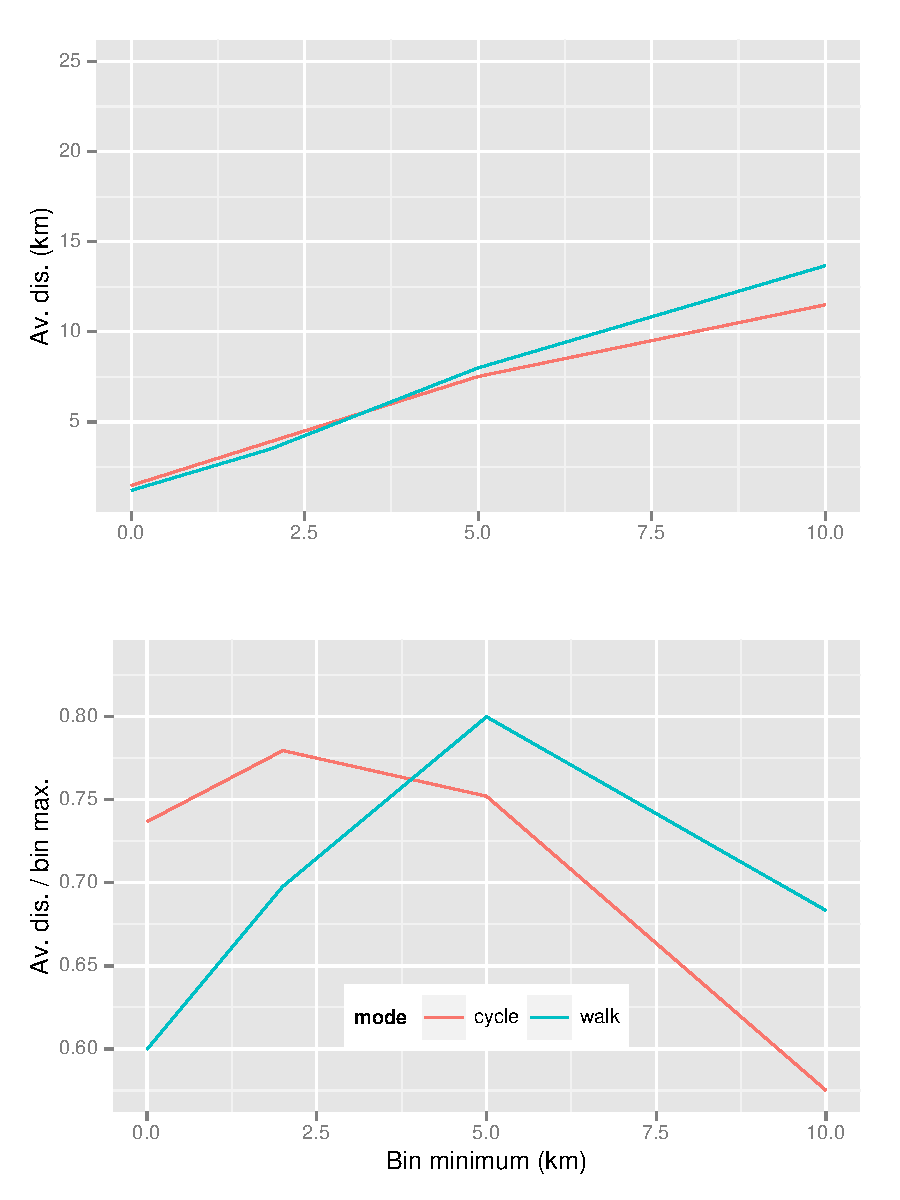
\includegraphics[width=9cm]{dboxes-walk}  \end{center}
  \caption[Distance bands and average distance travelled for active modes]
  {Distance bands and average distance travelled for non-motorised modes, expressed
  as the relationship between lower bound and average distance (top)
  and that between lower bound and the ratio of upper bound to average distance
  (below).} %%% could update with NTS!!! should have used centre...
 \label{fdboxes2}
\end{figure}

% As a result, it can be assumed that the number of commuter occupants in each
% car is 1 (so $EI_car$ = 2.98, not 2.4) for all those who
% ticked the option ``...'': Those who car share will be captured in option x:
% car passenger trips are counted a unique mode of transport to work. Calculated
% at the individual level, a sample of the input data and resulting values
% for Et are illustrated in table xx and xx for xxx, the first MSOA area in
% the input dataset.
% 
% Even if more accurate results can be obtained by, and assumptions behind, the data
% used to calculate energy costs per trip

Based on these categories, and the values of Ef reported in the previous section,
the 99 distance-mode variables of the cross-tabulated
census table ST121 can each be allocated an average energy
costs.
% !!! figure here right!
Originally the energy cost associated with the number of people in
each distance/mode category was calculated using the LibreOffice Calc
spreadsheet software. However, this soon became unwieldy so the analysis
was transferred into R. The main script file used to convert the raw
count data (\cref{frcount}) into energy estimates is available in the
`reproducible' folder associated with this
PhD.\footnote{Code
and output can also be embedded in RMarkdown, to ensure reproducible results.
Every step of this process is illustrated on the author's RPubs website
(\href{http://rpubs.com/RobinLovelace/7178}{rpubs.com/robinlovelace)}.}
The benefit of this script is that it can process input data of the type
displayed in \cref{frcount} and estimate energy use estimates broken-down by
mode and distance for each area, regardless of the number or scale of the
geographic units used.

Before 
% Starting at the largest (regional) geography, the results
% are displayed in \cref{fgoren} to \cref{fwarden}.

\section{Regional and sub-regional patterns} \label{sregional}
The average energy costs of commuter trips in England
are illustrated at the regional level in \cref{fgoren}, to provide an
overall impression of its spatial variability at the coarsest geography.
The high degree of geographical aggregation masks much of the variability,
yet there is still a substantial difference between regions. As expected,
London is the region with the lowest energy costs per commute at
20.8 MJ per one-way trip or 40\% below the average for all regions.
Excluding London, energy costs were lowest in the North West
and highest in the East of England (closely followed by the South East).
The variability between these regions was less noticeable:
they were 10\% below and 12\% below the national average respectively.


\begin{figure}[htbp]
\begin{center}
    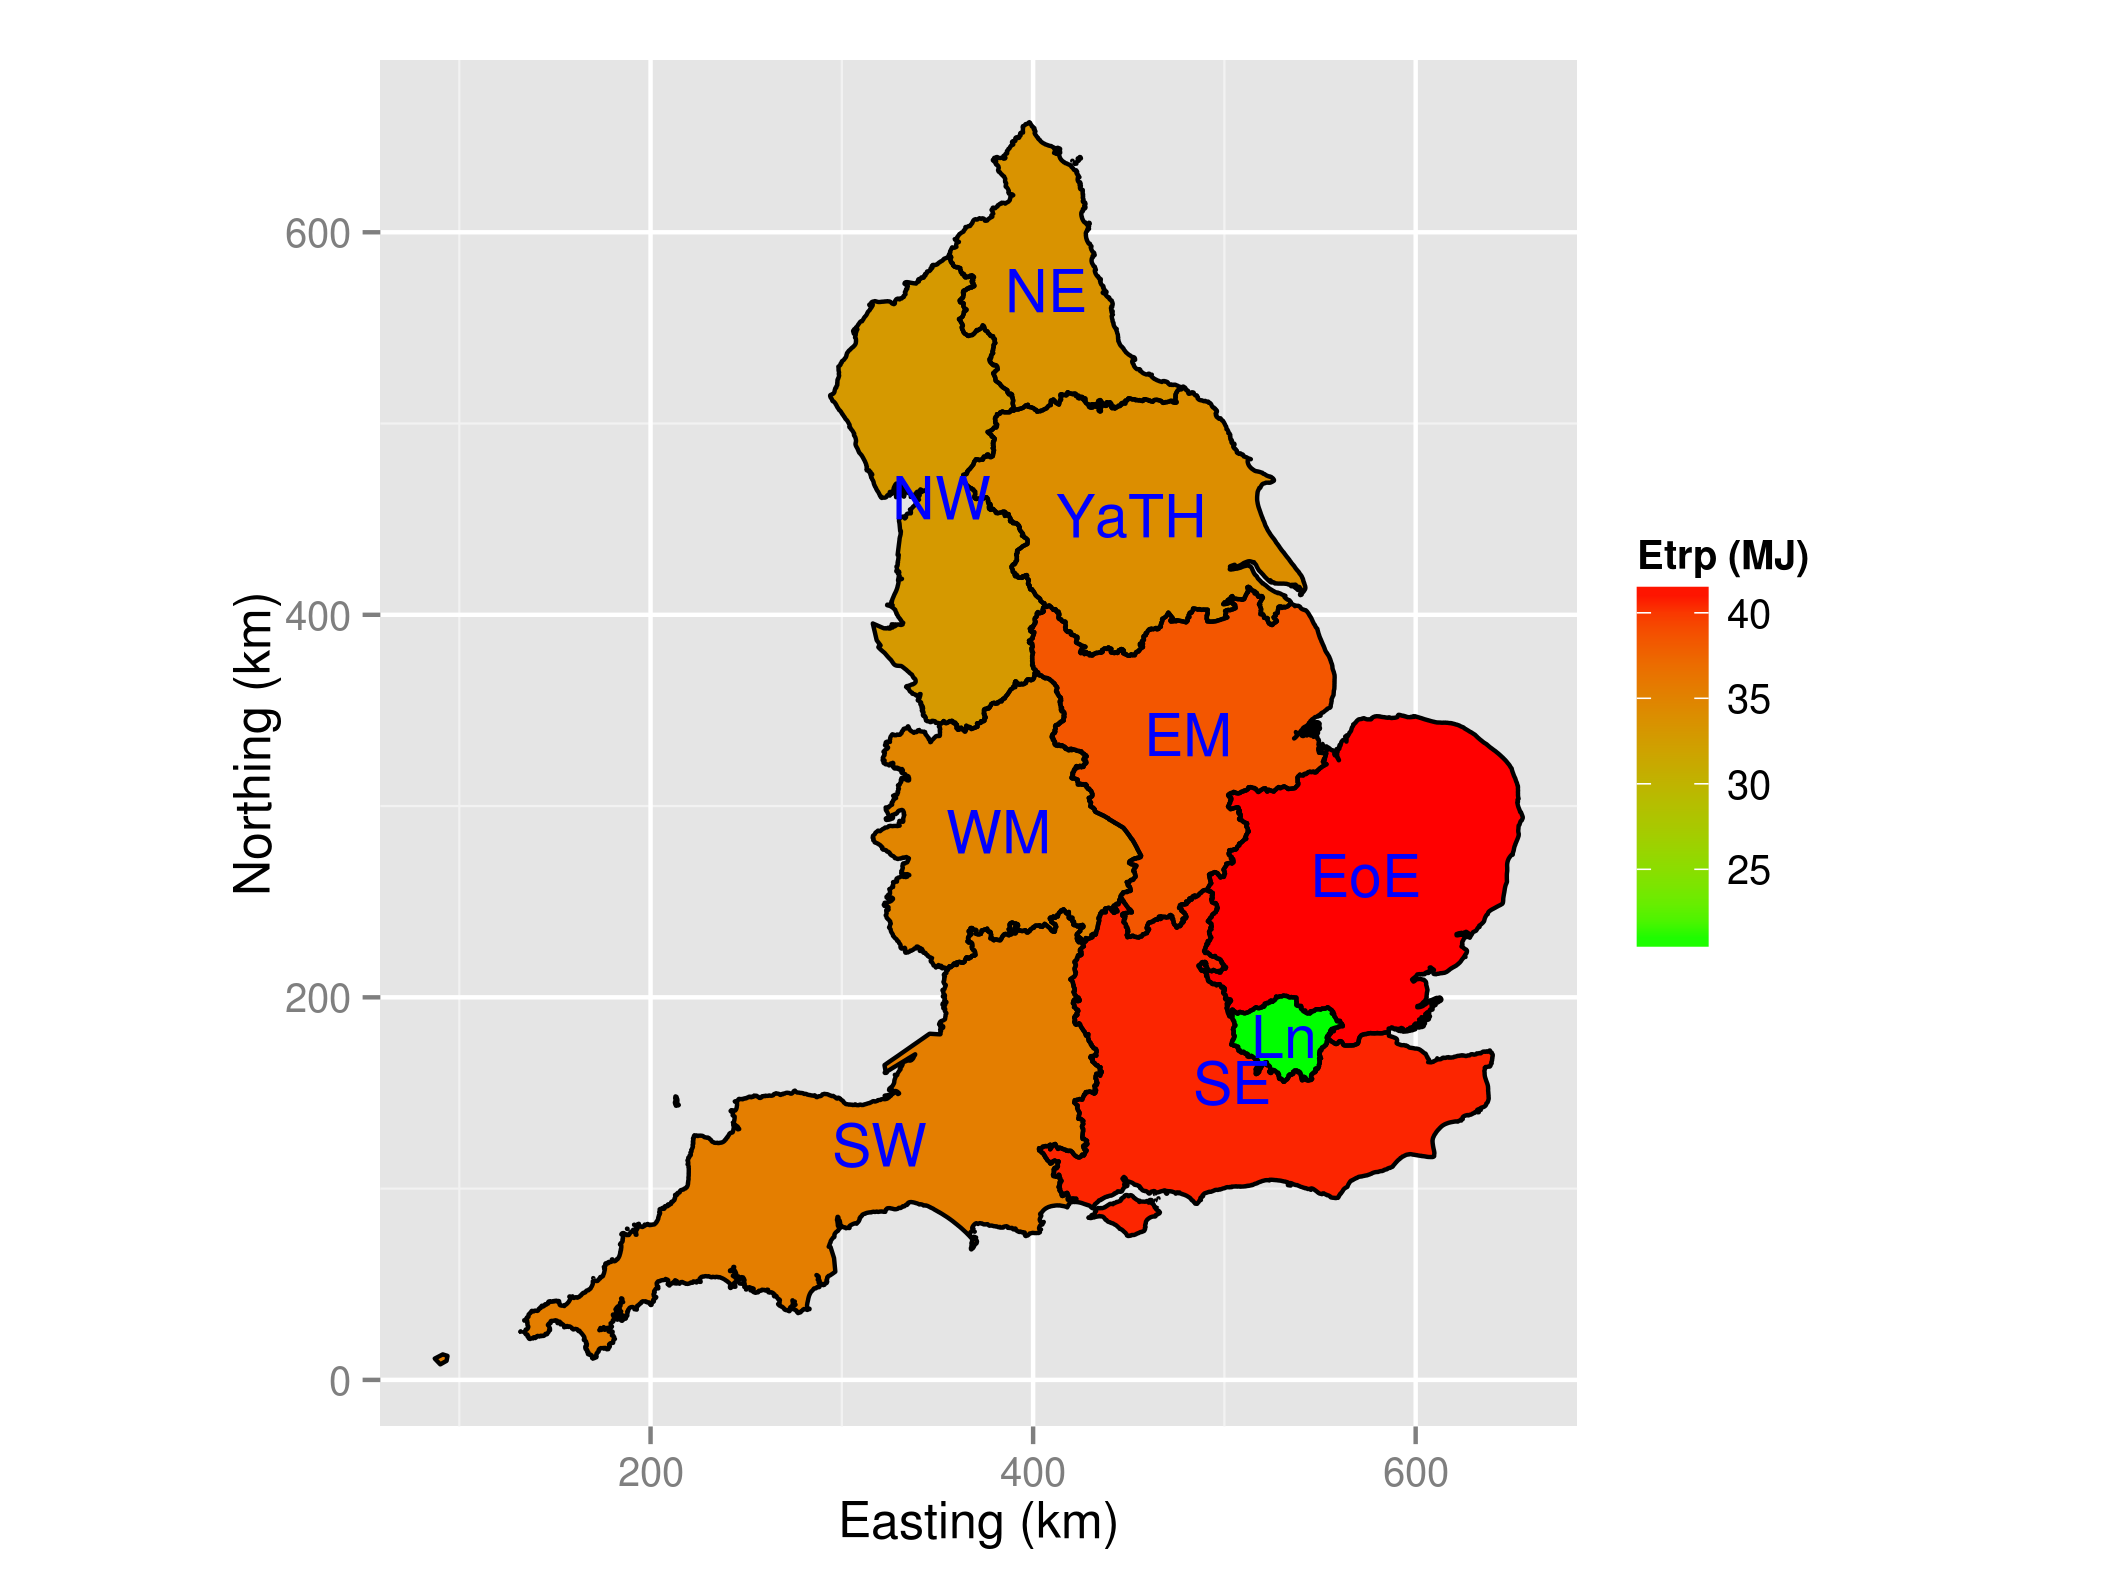
\includegraphics[width=10cm]{goren}  \end{center}
  \caption[Average energy use per trip (Etrp, in MJ) in English regions]
  {Average energy use per trip (Etrp, in MJ) in English regions, based
  on cross-tabulated distance/mode geographically aggregated count data}
 \label{fgoren}
\end{figure}

\begin{figure}[htbp]
\begin{center}
    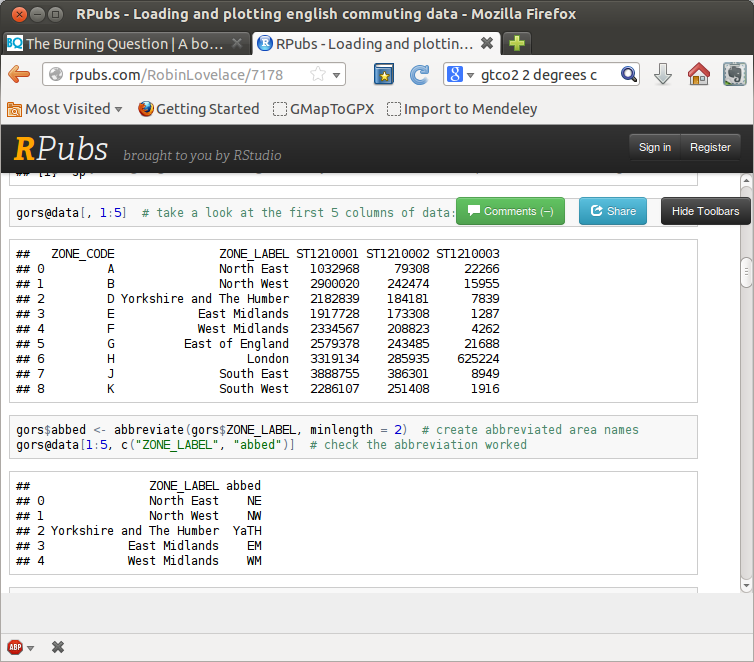
\includegraphics[width=13cm]{rawcount}  \end{center}
  \caption[Raw count data of commuters by mode and distance.]
  {Raw count data of commuters by mode and distance, the first 5 columns of
  regional level data, from Casweb table ST121. Data displayed in RMarkdown
  format, illustrating the reproducibility of the results (see
  \href{http://rpubs.com/robinlovelace}{www.RPubs.com}).}
 \label{frcount}
\end{figure}

To gain more insight into the spatial pattern of commuter energy costs,
the same data was re-plotted at lower geographical scales, down to the ward
level for the nation. \Cref{fcountyen} shows the distribution of energy costs
at the county level, constituting 88 polygons (42 counties and an additional 46
Local Authorities to make-up areas not covered by counties). This is a useful
level for identifying case study cities and areas that have unusually high
or low levels of energy use, given their surroundings. As a general pattern,
large and high-density urban areas tend to have lower energy use, with
the three largest built-up areas in England (Inner London, Greater Manchester
and the West Midlands built-up area) all having average commuter energy costs
below 30 MJ (the mean is 36). Another pattern that emerges is the relationship
between the very low energy costs of commuting in London, and the relatively high
costs of areas within a $\sim$100 km radius surround the centre: commuters in Bedford, Essex and
Kent, all of which contain `commuter belts' feeding London, for example, use
on average 45 MJ per trip to work. The highest and lowest (outside London)
values are found in Rutland (the geographic centroid of which is located 109
km from central London, and which was the last county in England to have
a direct trainline to London) the City of Kingston upon Hull.
Comparison of these two counties could make an interesting case study
to explore the reasons for underlying reasons behind high and low
energy costs of commuting in England.

\begin{figure}[htbp]
\begin{center}
    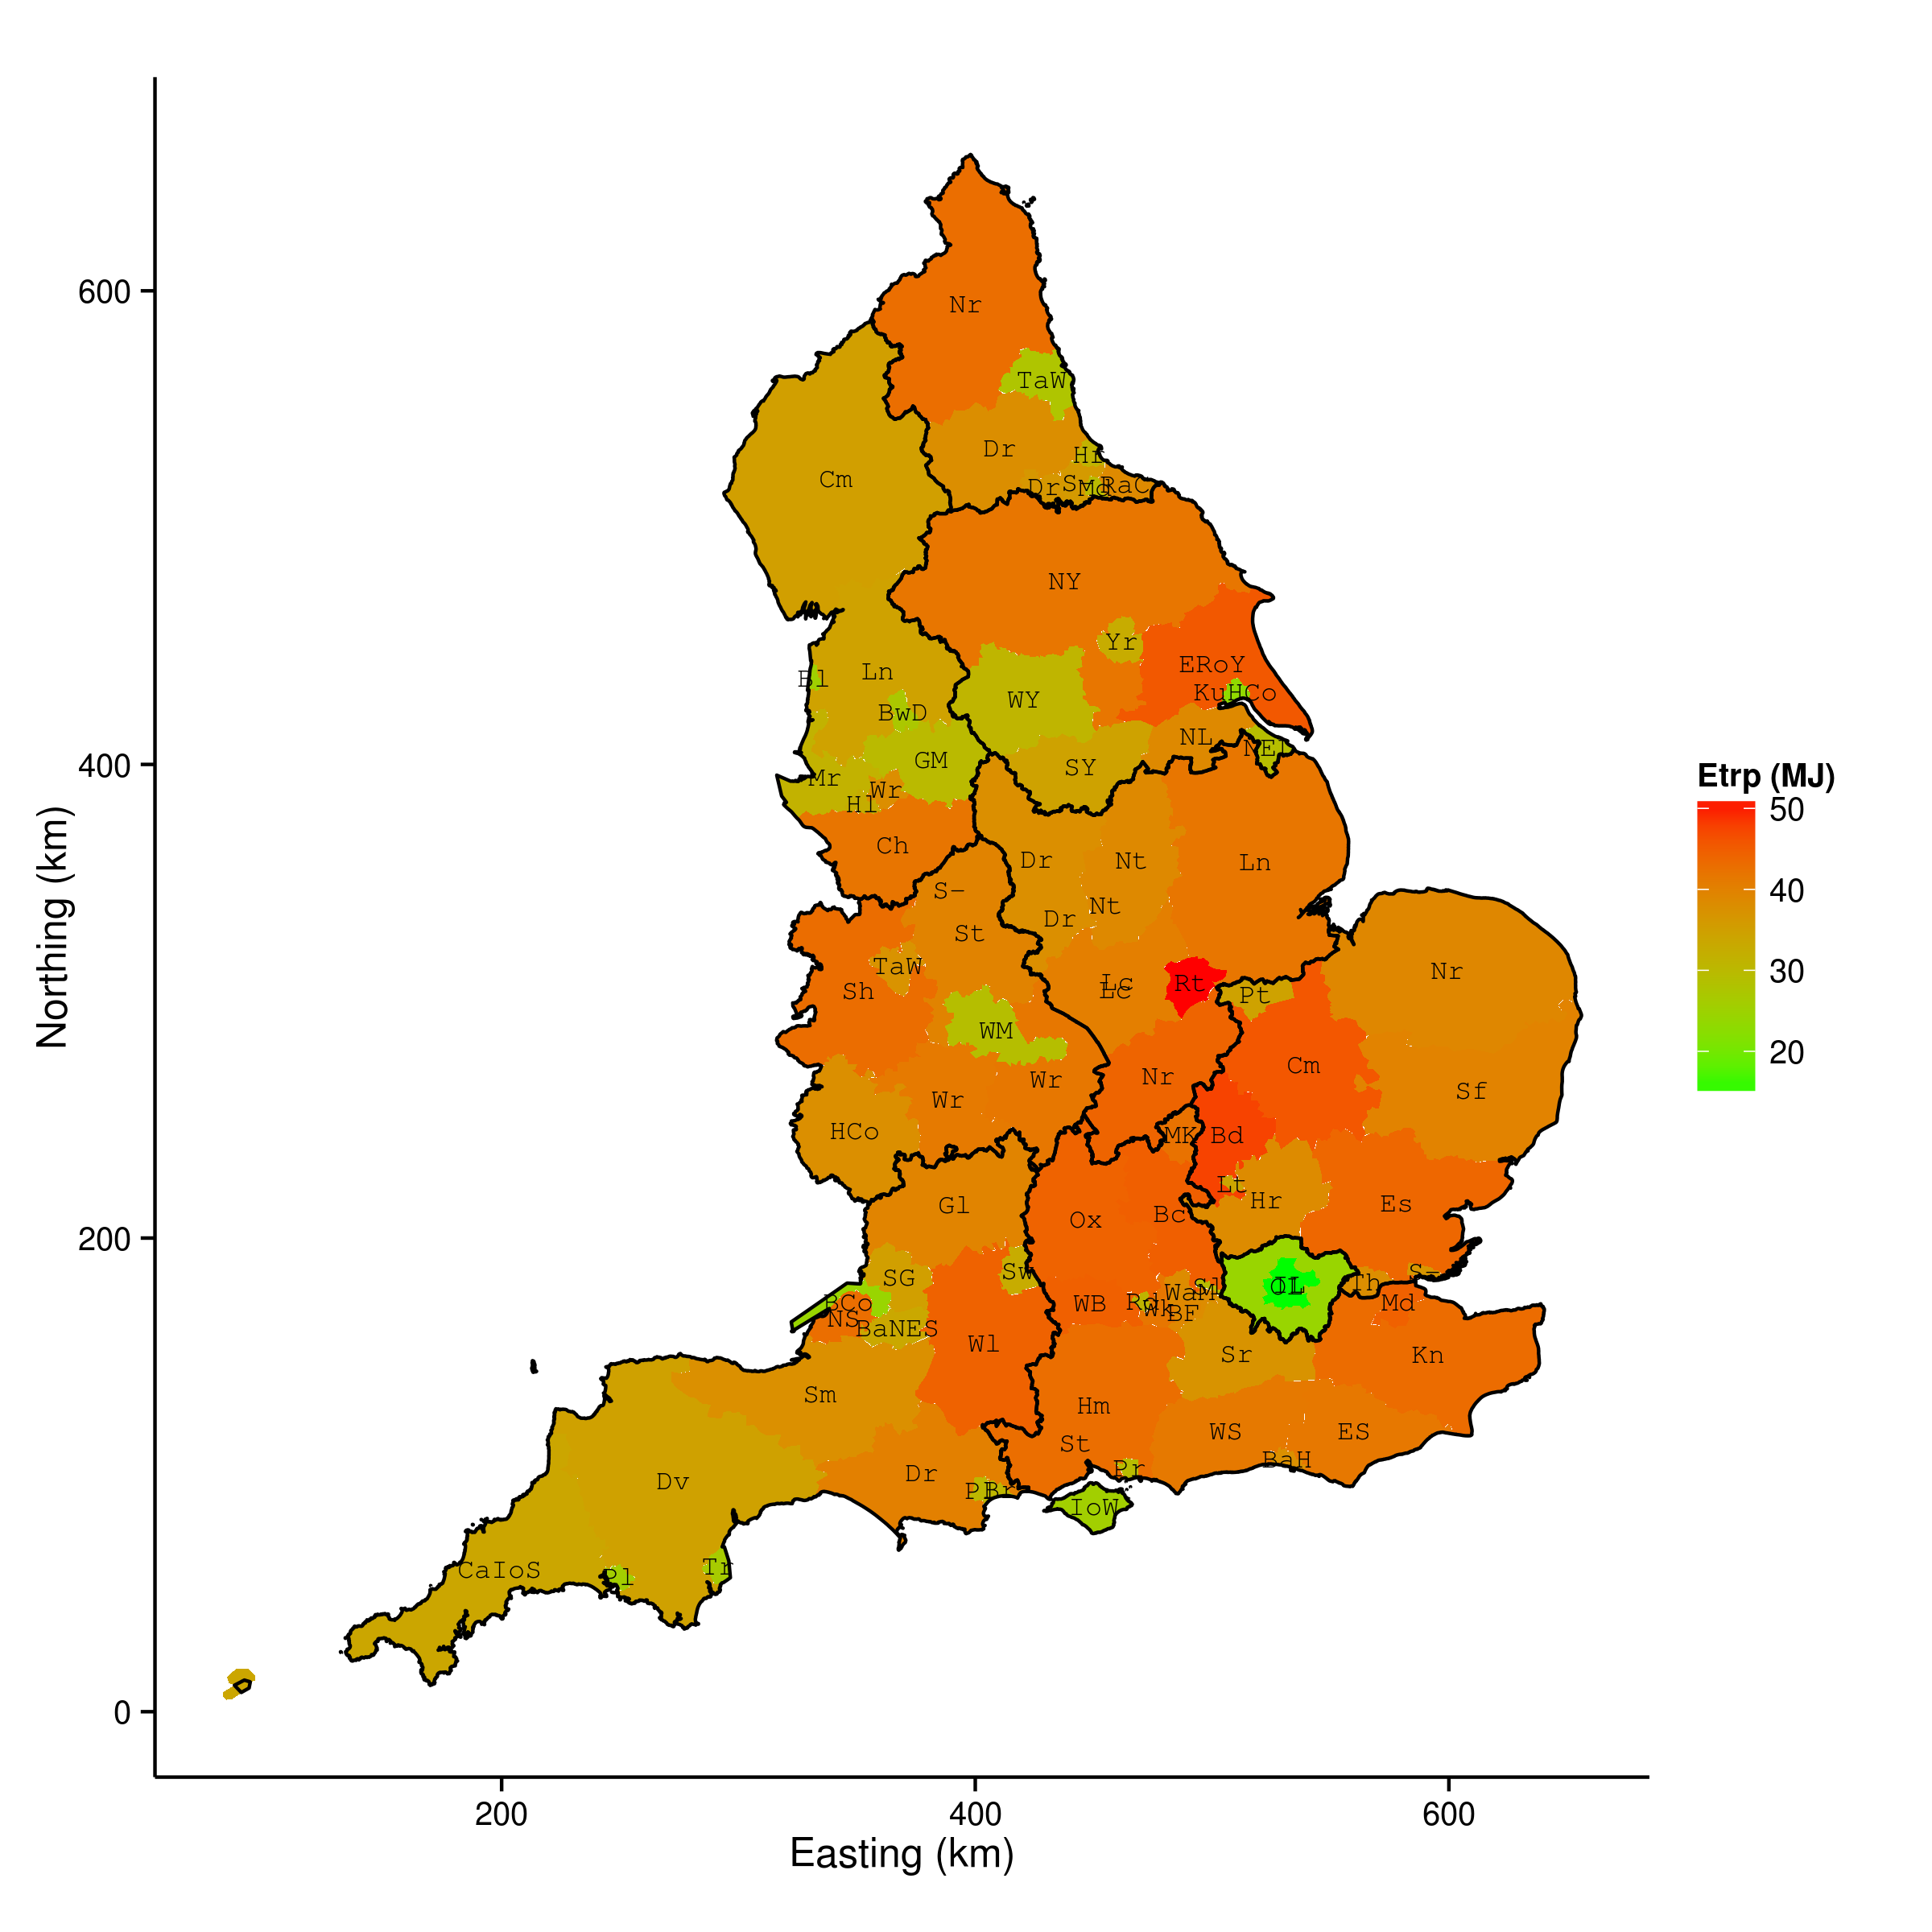
\includegraphics[width=13cm]{countyen}  \end{center}
  \caption[Average energy use per commuter trip at the county level]
  {Average energy use per commuter trip at the county level. The
  letter strings are abbreviations of the full county names (e.g. Dv is Devon).}
 \label{fcountyen}
\end{figure}

The results for districts, of which there are 308 in England,
are presented in \cref{fdistricten}.
As is apparent from the large and relatively homogeneous
area of bright green in London (and
knowing its high population density), the districts with the lowest
commuter energy costs are found in the capital. In fact,
9 out of 10 of the districts with the lowest energy costs per
commuter trip are located in London (the lowest is found in the
Isles of Scilly, with an average of 7.6 MJ/trip). The district with the
highest energy use per commuter trip (60 MJ/trip, 10\% more than the second
highest zone) is South Northamptonshire, visible
in \cref{fdistricten} as the red zone in the far south corner of the
East Midlands. The standard deviation of average energy use per trip at
this level of geographic aggregation was 9.0 MJ, 50\% higher than the
6.0 MJ/trip standard deviation observed at the regional level.

\begin{figure}[htbp]
\begin{center}
    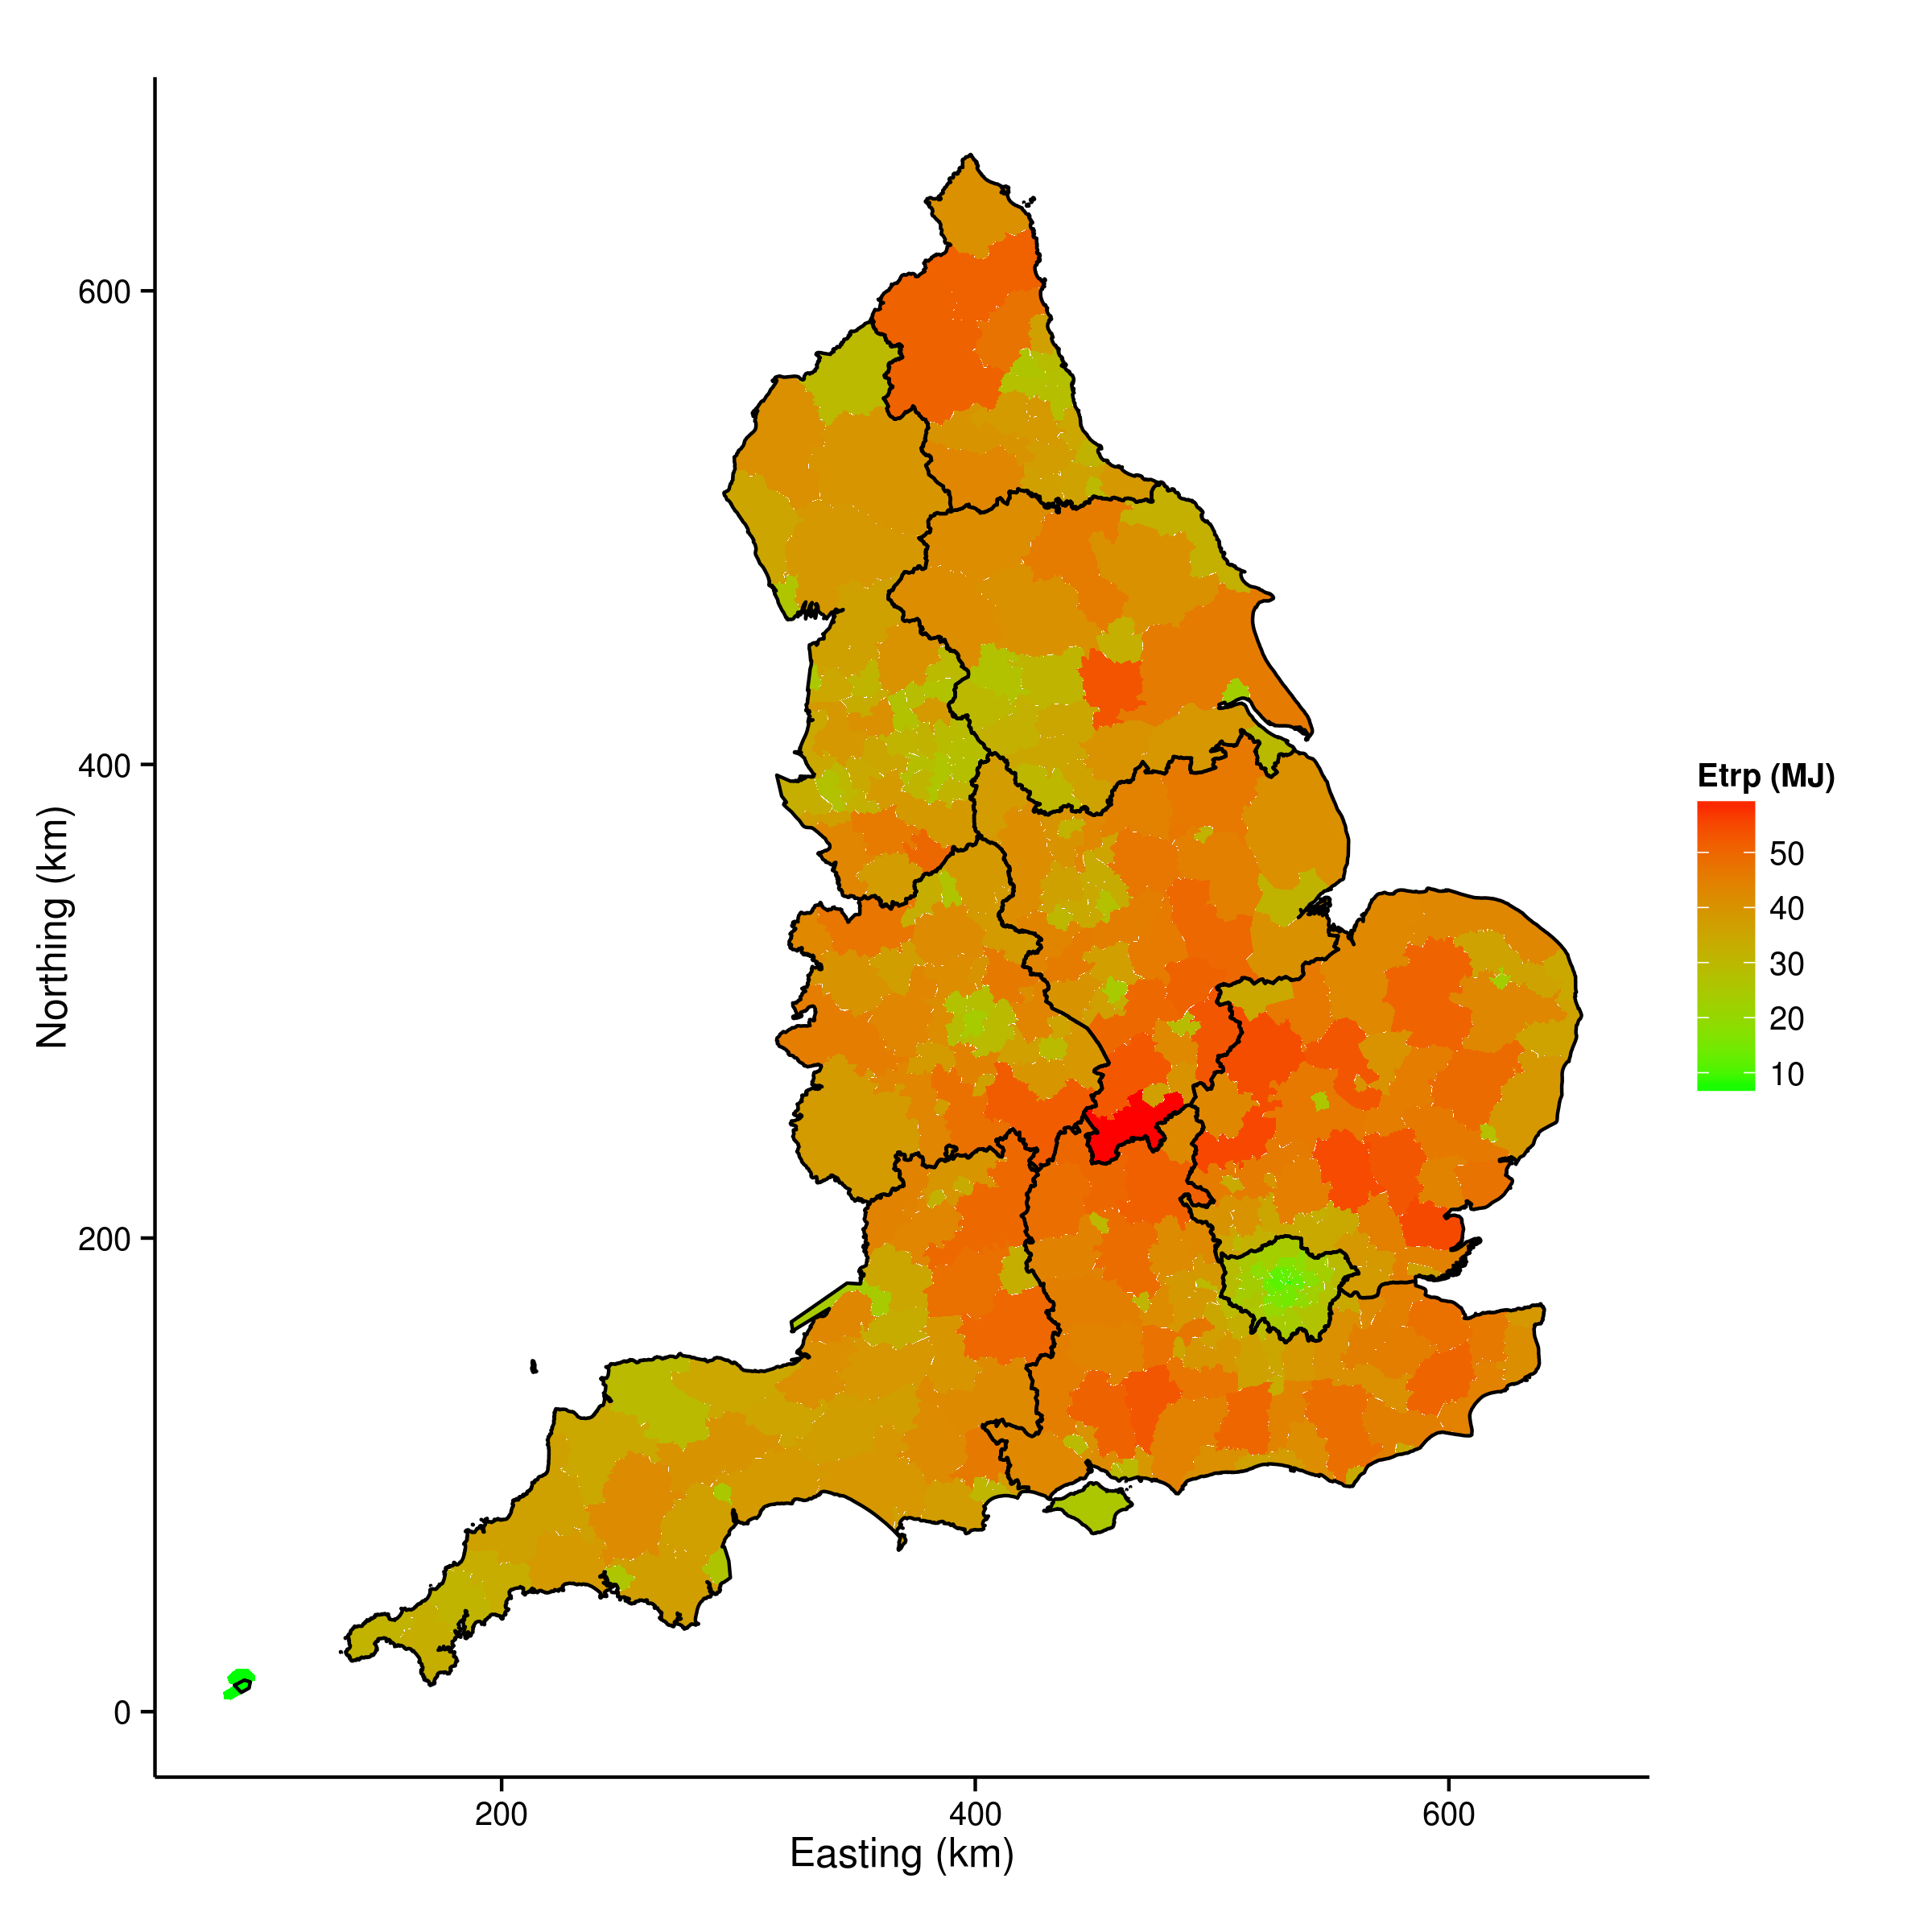
\includegraphics[width=13cm]{districten}  \end{center}
  \caption[Average energy use per commuter trip at the district level]
  {Average energy use per commuter trip at the district level.}
 \label{fdistricten}
\end{figure}

The same results are presented in \cref{fengplotnm}, at the ward level.
Here, much greater variability is apparent (note the increased range of
values represented in the colour scale). The standard deviation is 11.6
and values range all the way from 5.1 to 88 MJ per trip.
It is interesting to not where these extreme values are found:
the former is located in the central London ward of
Portsoken, where walking is the most common mode of travel to work,
followed closely by catching the tram. The latter was
found in in Park Farm North,
a suburban ward located in the far South East of England, just south of
Ashford, where car drivers account for 68\% of all commutes. The complex
patchwork of average  commuter energy costs displayed in \cref{fengplotnm}
suggests that regional level assessments, such as those
presented in \cref{fgoren}, are not able to capture the full geographical
variability of the variable at all well: there is much more variability
within zones than between them. One pattern that stands out from the ward level
analysis is the tendency of settlements to be directly surrounded by green areas
associated with low energy costs. Although only large cities (those with
populations in excess of 100,000) are displayed in
\cref{fengplotnm}, it seems that many towns and cities are immediately surrounded
by areas of low commuter energy costs. Haverhill (located in the East of
England, roughly half-way between Cambridge and Chelmsford),
Hereford (in the south-west of the West Midlands) and a number of coastal
towns such as  Sheringham ($\sim$40 km north of Norwich) and Scarborough
(in Yorkshire and the Humber) are examples of this.
%%% Link here to analysis showing cor between remoteness and ecosts
\begin{figure}[htbp]
\begin{center}
    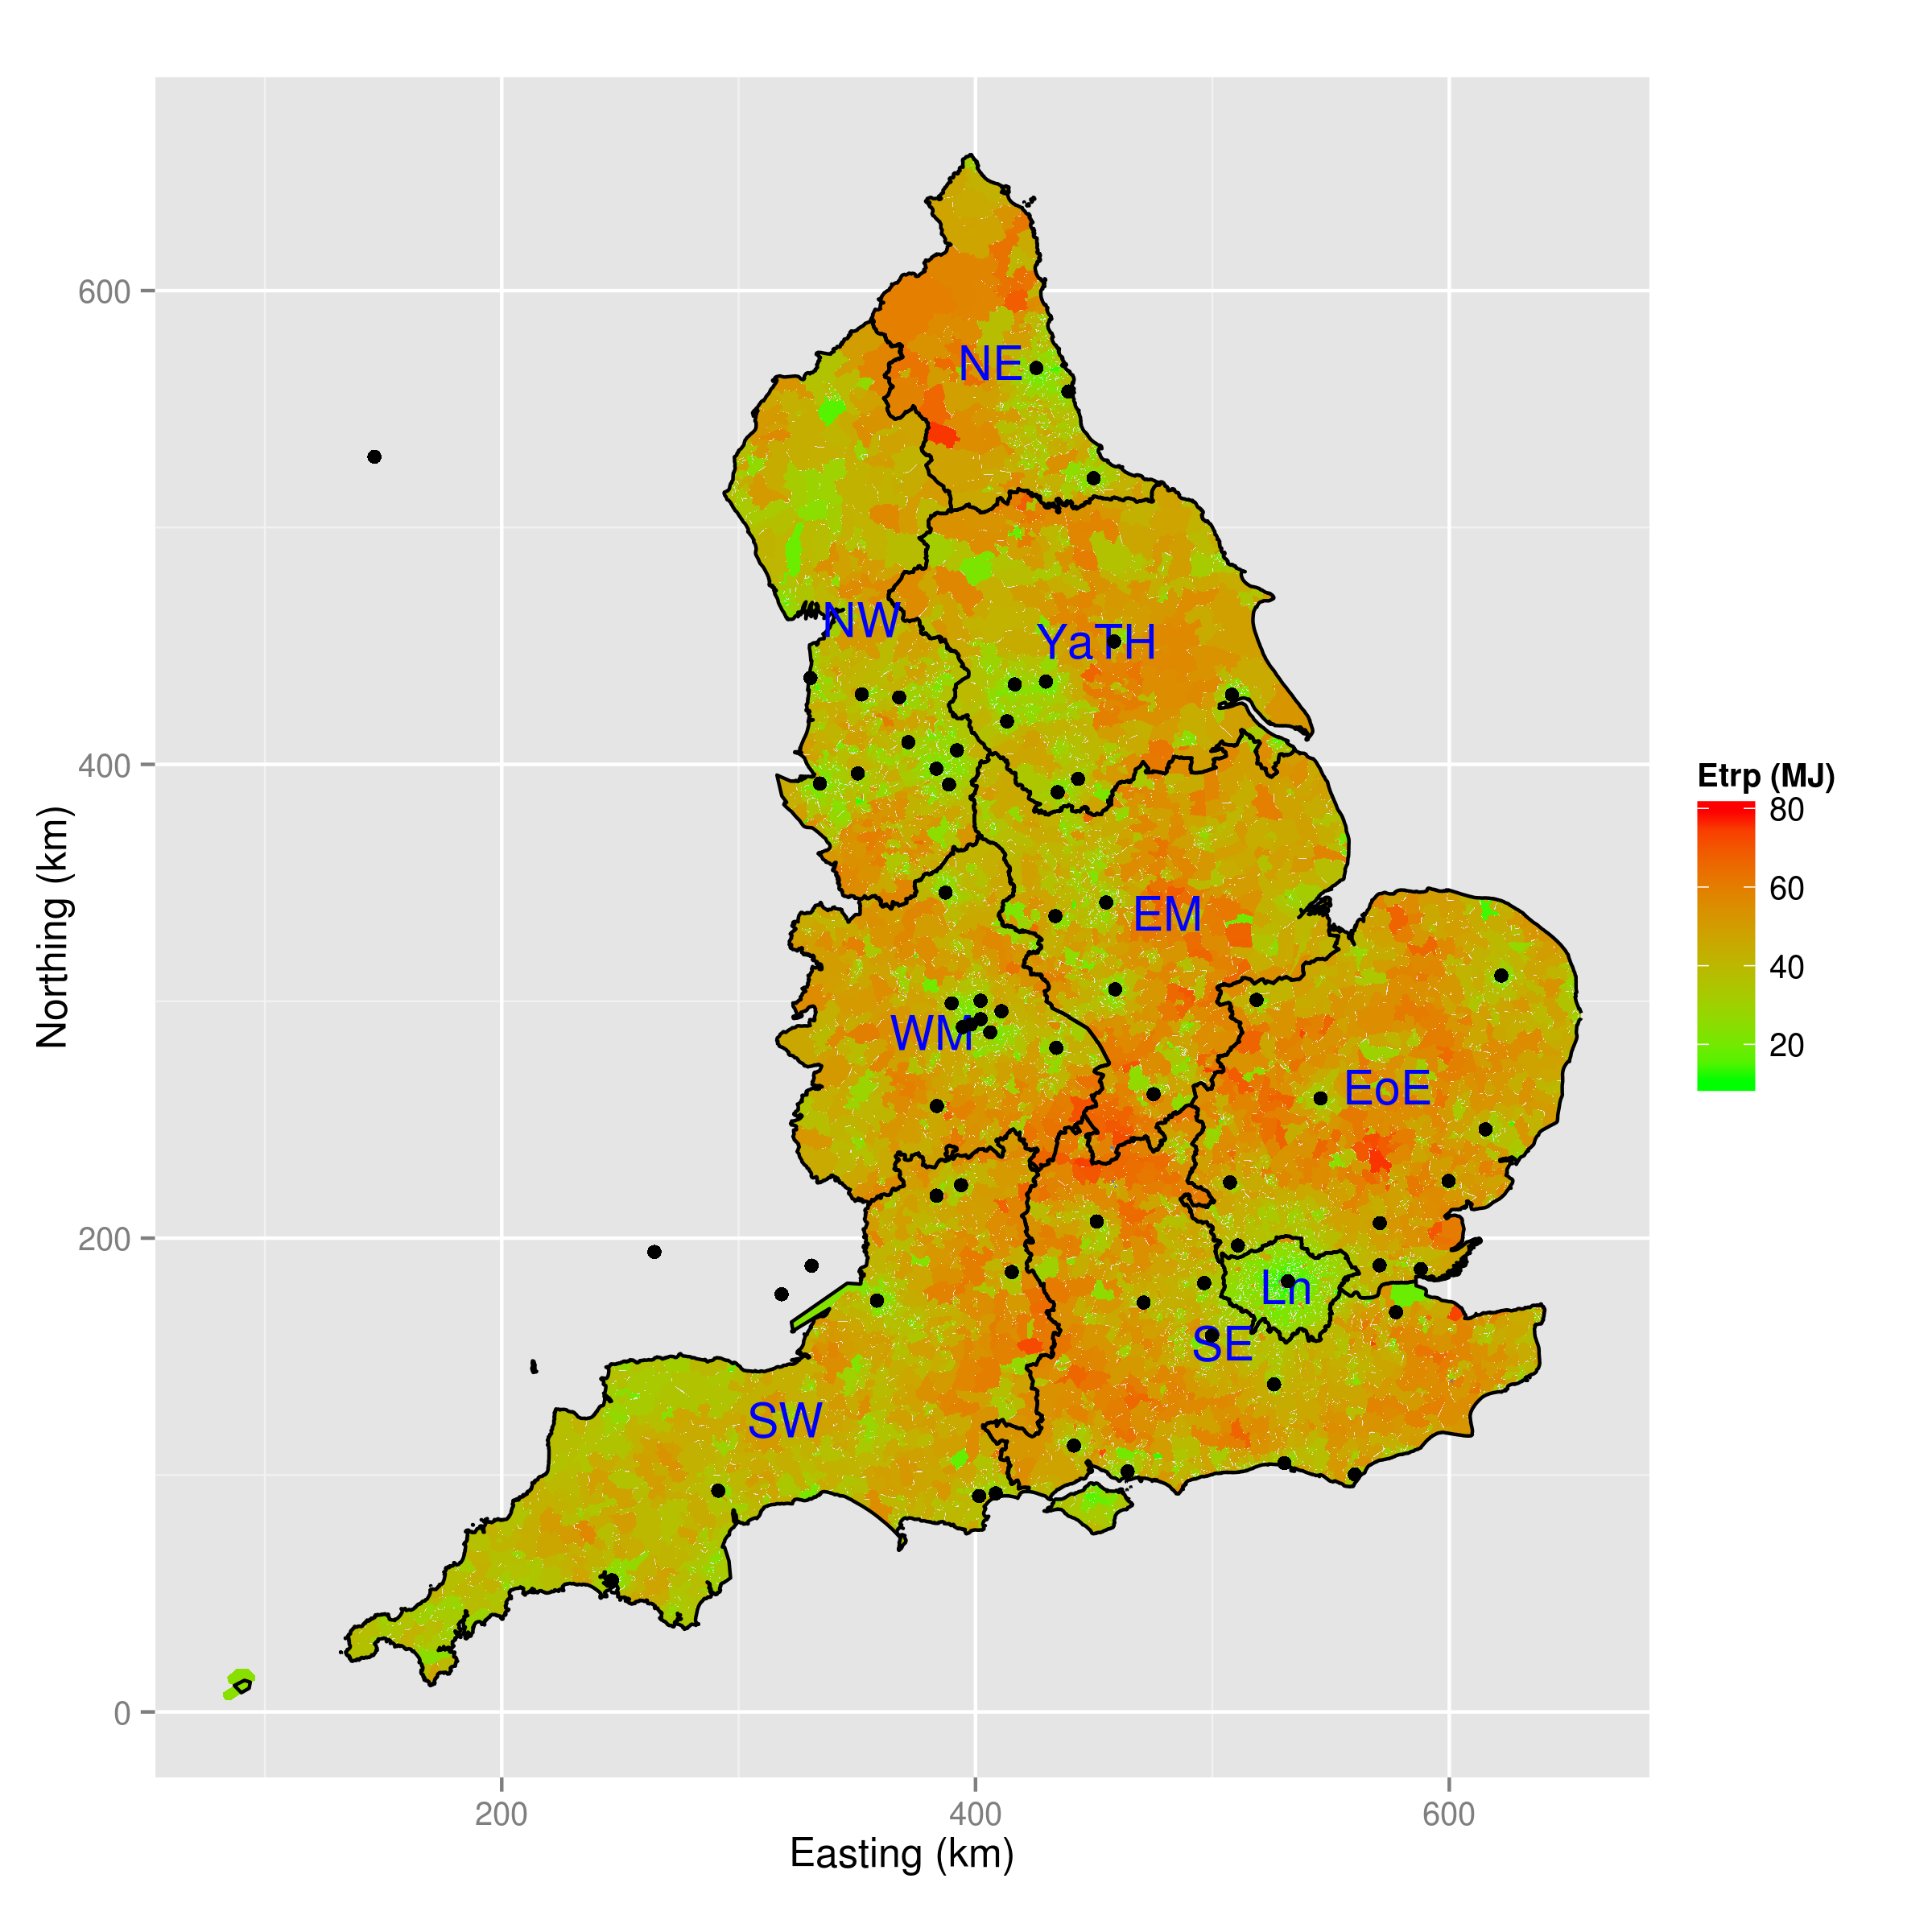
\includegraphics[width=16cm]{engplotnm}  \end{center}
  \caption[Average energy use per trip (Etrp, in MJ) in English wards]
  {Average energy use per trip (Etrp, in MJ) in English wards.
  The black dots are large (100,000 people or more) cities (from
  \citet{Brownrigg2013}).}
 \label{fengplotnm}
\end{figure}

The method used to calculate energy costs creates estimates
calculations that are dis-aggregated by mode and distance. This allows the
aggregate energy use result in each area to be subdivided.
A policy-relevant example of this would be those areas in which
short-distance car journey constitute
a large proportion of the energy costs of work travel (these areas
may benefit from improved walking and cycling infrastructure). Another example
is the proportion of commuter trip energy use
in each area used by trains. The result is interesting in itself, and
provides confidence that the calculations are working correctly:
it is clear from \cref{ftrainen} that there is a tendency for
areas located close to be associated with a high proportion of per trip energy
use to be composed of rail travel. Also as expected, areas with fast rail
connections to London seem to have high energy use for this mode of travel.

\begin{figure}[htbp]
\begin{center}
    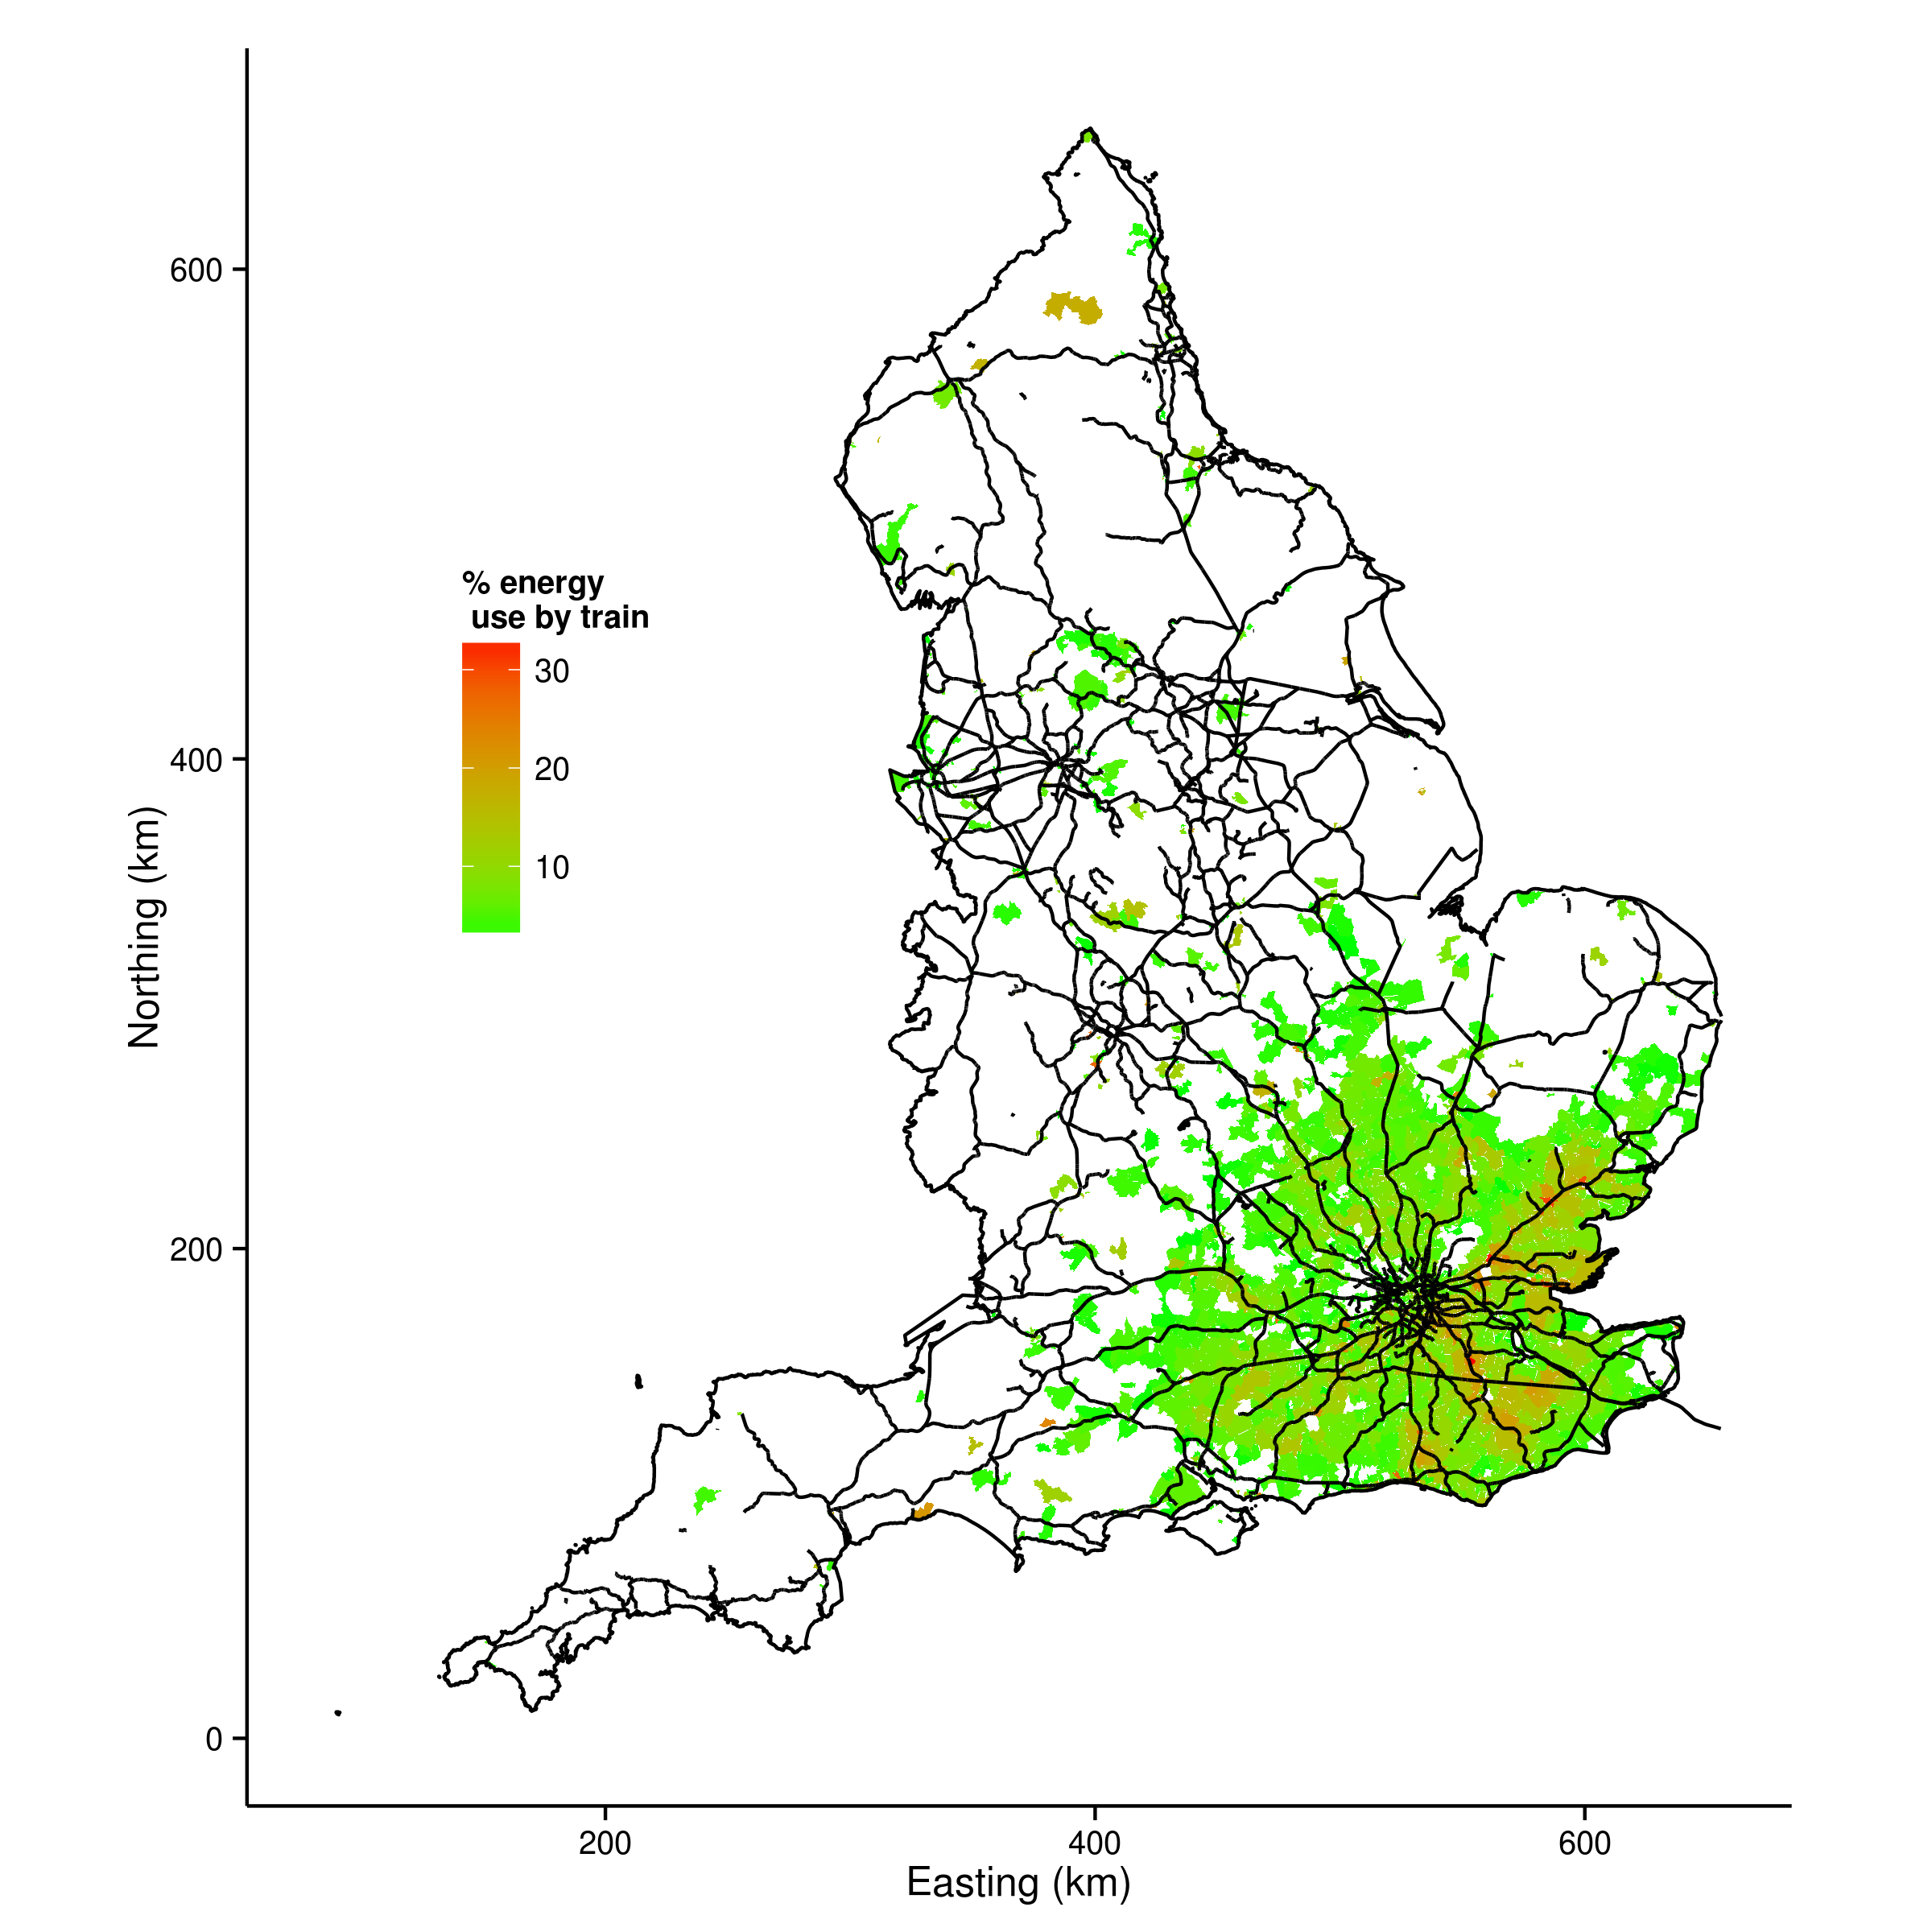
\includegraphics[width=16cm]{trainen}  \end{center}
  \caption[Proportion of energy use caused by train trips]
  {Proportion of energy use caused by train trips. Only areas
  above the national average (3\%) are plotted.}
 \label{ftrainen}
\end{figure}

\section{Local and individual level variability} \label{sindvar}

As with any research in which geographical zones are the unit of analysis,
the maps of energy use presented above mask individual level variability within
zones. If interpreted incorrectly, conclusions resulting from such analyses
may be `ecological fallacies', where knowledge generated
at one level of understanding is incorrectly applied to another.
To provide an example, the strength of the correlation between wealth and the energy
costs of work travel at the ward level is unlikely to be the same as the
strength of the correlation at the level of individuals. The process of
geographic aggregation smooths relationships, often making correlations seem
greater and simpler that they really are \citep{Openshaw1983}. 

Spatial microsimulation can also be used to generate estimates of
geographically aggregated variables such as income, hence the use of the term
`small area estimation' used to describe some spatial microsimulation models
(see \cref{Chapter3}). Regarding the energy use of travel to work, spatial
microsimulation can help overcome a major data constraint at some geographical
levels: energy use is roughly a function of mode and distance of travel, yet
in some cases no cross tabulations on this matter are provided.
Even if average distances of travel to work are provided, it may be
impossible to know which modes of travel are responsible for high values.
When distance band and mode of travel are know but no cross-tabulations
are provided between them (as is the case with Super Output Area administrative
geographical levels from the data portal Casweb),
spatial microsimulation can be used to `fill in the gaps'.


A final potential issue with the ward level analysis of the entire nation, as presented
above, is the assumption that relationships are constant over space.
In many cases this assumption may justified (e.g. for the relationship between
population density and travel-to-work distance, which can be assumed to be
more-or-less universal), but sometimes relationships vary
substantially from place to place. This is a central motivation behind
geographically weighted regression \citep{Fotheringham2002}.

\subsection{A case study from South Yorkshire}
To illustrate the results of the spatial microsimulation model
in terms of energy use, we will focus on South Yorkshire.
There is no strong justification for this choice of case study
area:
the purpose is to illustrate the kinds of result that the
spatial microsimulation method can generate. In addition,
South Yorkshire is used in the subsequent chapter as the case study region
for illustrating the potential of the methods to explore social and spatial
inequalities, for continuity between chapters.
Because the majority of the analysis was done in R (with the R's
improving geo-spatial data handling packages, all of the analysis
could be done in this environment), some of the results are
reported as listings, to illustrate how the results are accessed.

After running the spatial microsimulation model outlined in
\cref{Chapter4}, constraining by age/sex, mode, distance of commute and
social class, an R object called a list is created. The list is a collection
of data tables, one for each administrative zone; each contains a number of
rows corresponding to the number of commuters in the area of interest.
The results for the first six individual in the first MSOA area
in South Yorkshire in the list (``Barnsley 001'') are displayed in
\cref{tintallh}.

\begin{table}[htbp]
\caption[Sample of the spatial microsimulation model output]
{Sample of the spatial microsimulation model output for South
Yorkshire. The table was saved as a comma-delimited file with the command
``intall[[1]]'', which refers to the data table corresponding to the
first zone in Sheffield. In total, the R object
``intall'' contains 532,130 individuals from 176 MSOA zones.}
\begin{tabular}{rrrrlrrlllr}
\toprule
\multicolumn{1}{l}{} & \multicolumn{1}{l}{a\_hidp} & \multicolumn{1}{l}{a\_pno} &
\multicolumn{1}{l}{pidp} & sex & \multicolumn{1}{l}{age} & \multicolumn{1}{l}{dis}
& mode & nssec8 & urb & \multicolumn{1}{l}{ncars} \\
\midrule
18 & 68041483 & 2 & 68041491 & male & 35 & 71 & Car (d) & Other & rural & 2 \\
18 & 68041483 & 2 & 68041491 & male & 35 & 71 & Car (d) & Other & rural & 2 \\
200 & 68303283 & 1 & 68303287 & male & 41 & 125 & Car (d) & Other & urban & 1 \\
200 & 68303283 & 1 & 68303287 & male & 41 & 125 & Car (d) & Other & urban & 1 \\
219 & 68323003 & 1 & 68323007 & male & 53 & 71 & Car (d) & Other & urban & 1 \\
219 & 68323003 & 1 & 68323007 & male & 53 & 71 & Car (d) & Other & urban & 1 \\
\bottomrule
\end{tabular}
\label{tintallh}
\end{table}

From the household and personal ids (a\_hidp and a\_pidp) can be joined a
wide range of additional variables (\cref{tintcar}).
Binding the information representing
in \cref{tintallh} for all 176 zones (using the command \verb do.call() )
results in a single table representing all five hundred thousand commuters
in South Yorkshire. From here, energy use data can be produced for each
individual, using the same technique described for the calculation of
aggregate energy use. The additional refinement added at this individual level
was the size of car: large cars were allocated a higher value (3.9 MJ/km)
than small cars (2.5 MJ/km).\footnote{13.6\% of
responses to this question were ``inapplicable'' or some other `NA' value,
even amongst those who drove a car. In these cases the energy costs were
set equal to those of a medium-sized car.}
\begin{table}[htbp]
\caption[Sample of individual level spatial microsimulation output]
{Sample of individual level microsimulation output. The number of cars
in the individuals' household and the engine size of their primary car
are extracted using the merge() ~function applied to the ID codes,
that are also present in \cref{tintallh}}
\begin{tabular}{rrrrrlr}
\toprule
\multicolumn{1}{l}{} & \multicolumn{1}{l}{a\_hidp} & \multicolumn{1}{l}{a\_pno} & \multicolumn{1}{l}{pidp} & \multicolumn{1}{l}{N.~cars} & Engine size & \multicolumn{1}{l}{Et} \\ \midrule
18 & 68041483 & 2 & 68041491 & 2 Sheffield& medium engine - 1.4 - 1.9999 & 312.3 \\
18 & 68041483 & 2 & 68041491 & 2 & small engine - 1.0 - 1.3999 & 268.3 \\
200 & 68303283 & 1 & 68303287 & 1 & inapplicable & 743.8 \\
200 & 68303283 & 1 & 68303287 & 1 & small engine - 1.0 - 1.3999 & 471.7 \\
219 & 68323003 & 1 & 68323007 & 1 & inapplicable & 423.0 \\
219 & 68323003 & 1 & 68323007 & 1 & medium engine - 1.4 - 1.9999 & 312.3 \\
\bottomrule
\end{tabular}
\label{tintcar}
\end{table}

The impact of car engine size on the relative average energy use of each
zone was found to be very small and the correlation between values calculated
that did not take car size into account and values that did was very high
(r = 0.9985). The resulting spatial distribution of energy costs of
commuting at the MSOA level is plotted in \cref{fsoyoen}. This illustrates how
spatial microsimulation can be used to create estimates of energy use at the
aggregate level when cross-tabulated distance/mode data is unavailable.
At the individual level, the standard deviation in per trip
energy use is much greater than at the geographical level in this
case study: 95 MJ between individuals compared with only 11 MJ between
MSOA areas. This reflects the impact of geographical smoothing and also
provides an indication of the high level of inequality in energy use for
work travel between commuters living in the same area.

\begin{figure}[htbp]
\begin{center}
    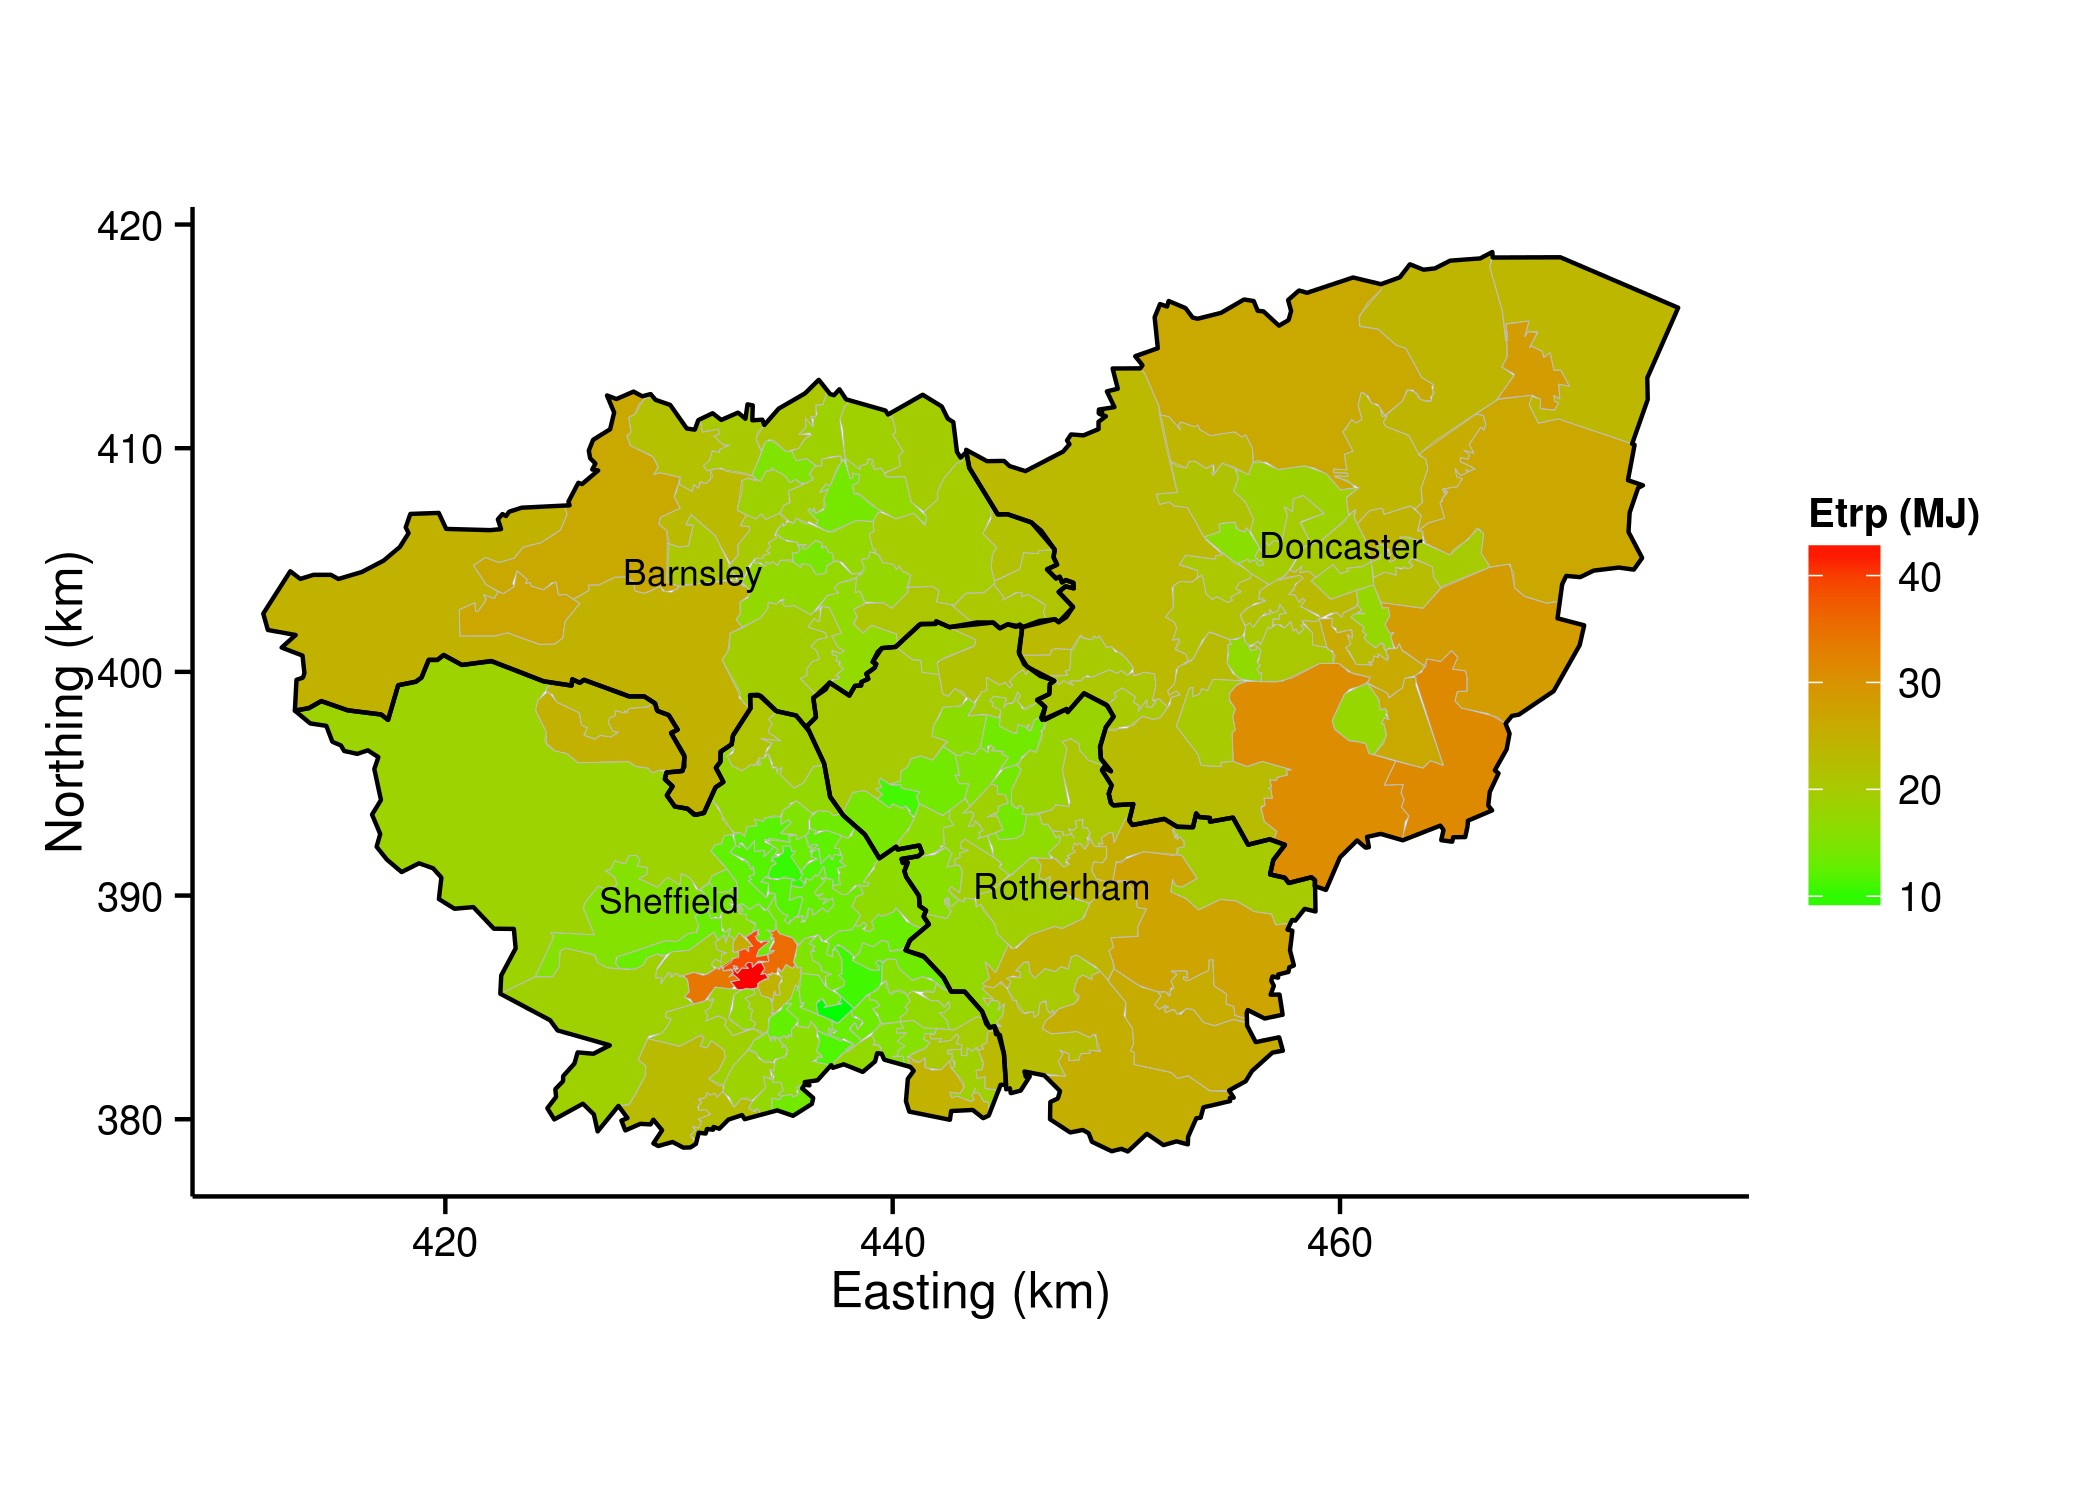
\includegraphics[width=14cm]{soyoen}  \end{center}
  \caption[Energy use per commuter trip at the MSOA level in South Yorkshire]
  {Energy use at the MSOA level in South Yorkshire.}
 \label{fsoyoen}
\end{figure}

The individual level results are well-illustrated by plotting the proportion
of energy use consumed by different groups. The example plotted in
\cref{fineq20} represents the proportion of energy use for commuting
consumed by the 20\% most energy-intensive commuters, which is also a
proxy for inequality. This plot shows a very clear spatial pattern,
with city centres being associated with the most unequal distribution
of commuter energy costs. We will return to this point in the subsequent
chapter --- for now suffice to say it is an interesting result.
To illustrate the method's ability to disaggregate
by socio-economic categories, \cref{ftopprop} shows the ratio of energy
used for commuting by the top social classes (1.1 and 1.2) compared with
the average energy cost per commute in each area. It is interesting to
note that in all areas the value is above 1.4, reaching more than 3 times
the average in some areas. More detailed analysis at the individual
level is presented in \cref{Chapter7}. The results presented in this section
demonstrate that individual level variability in commuter energy use
is important and in some cases potentially more so than inter-zone variation.

\begin{figure}[htbp]
\begin{center}
    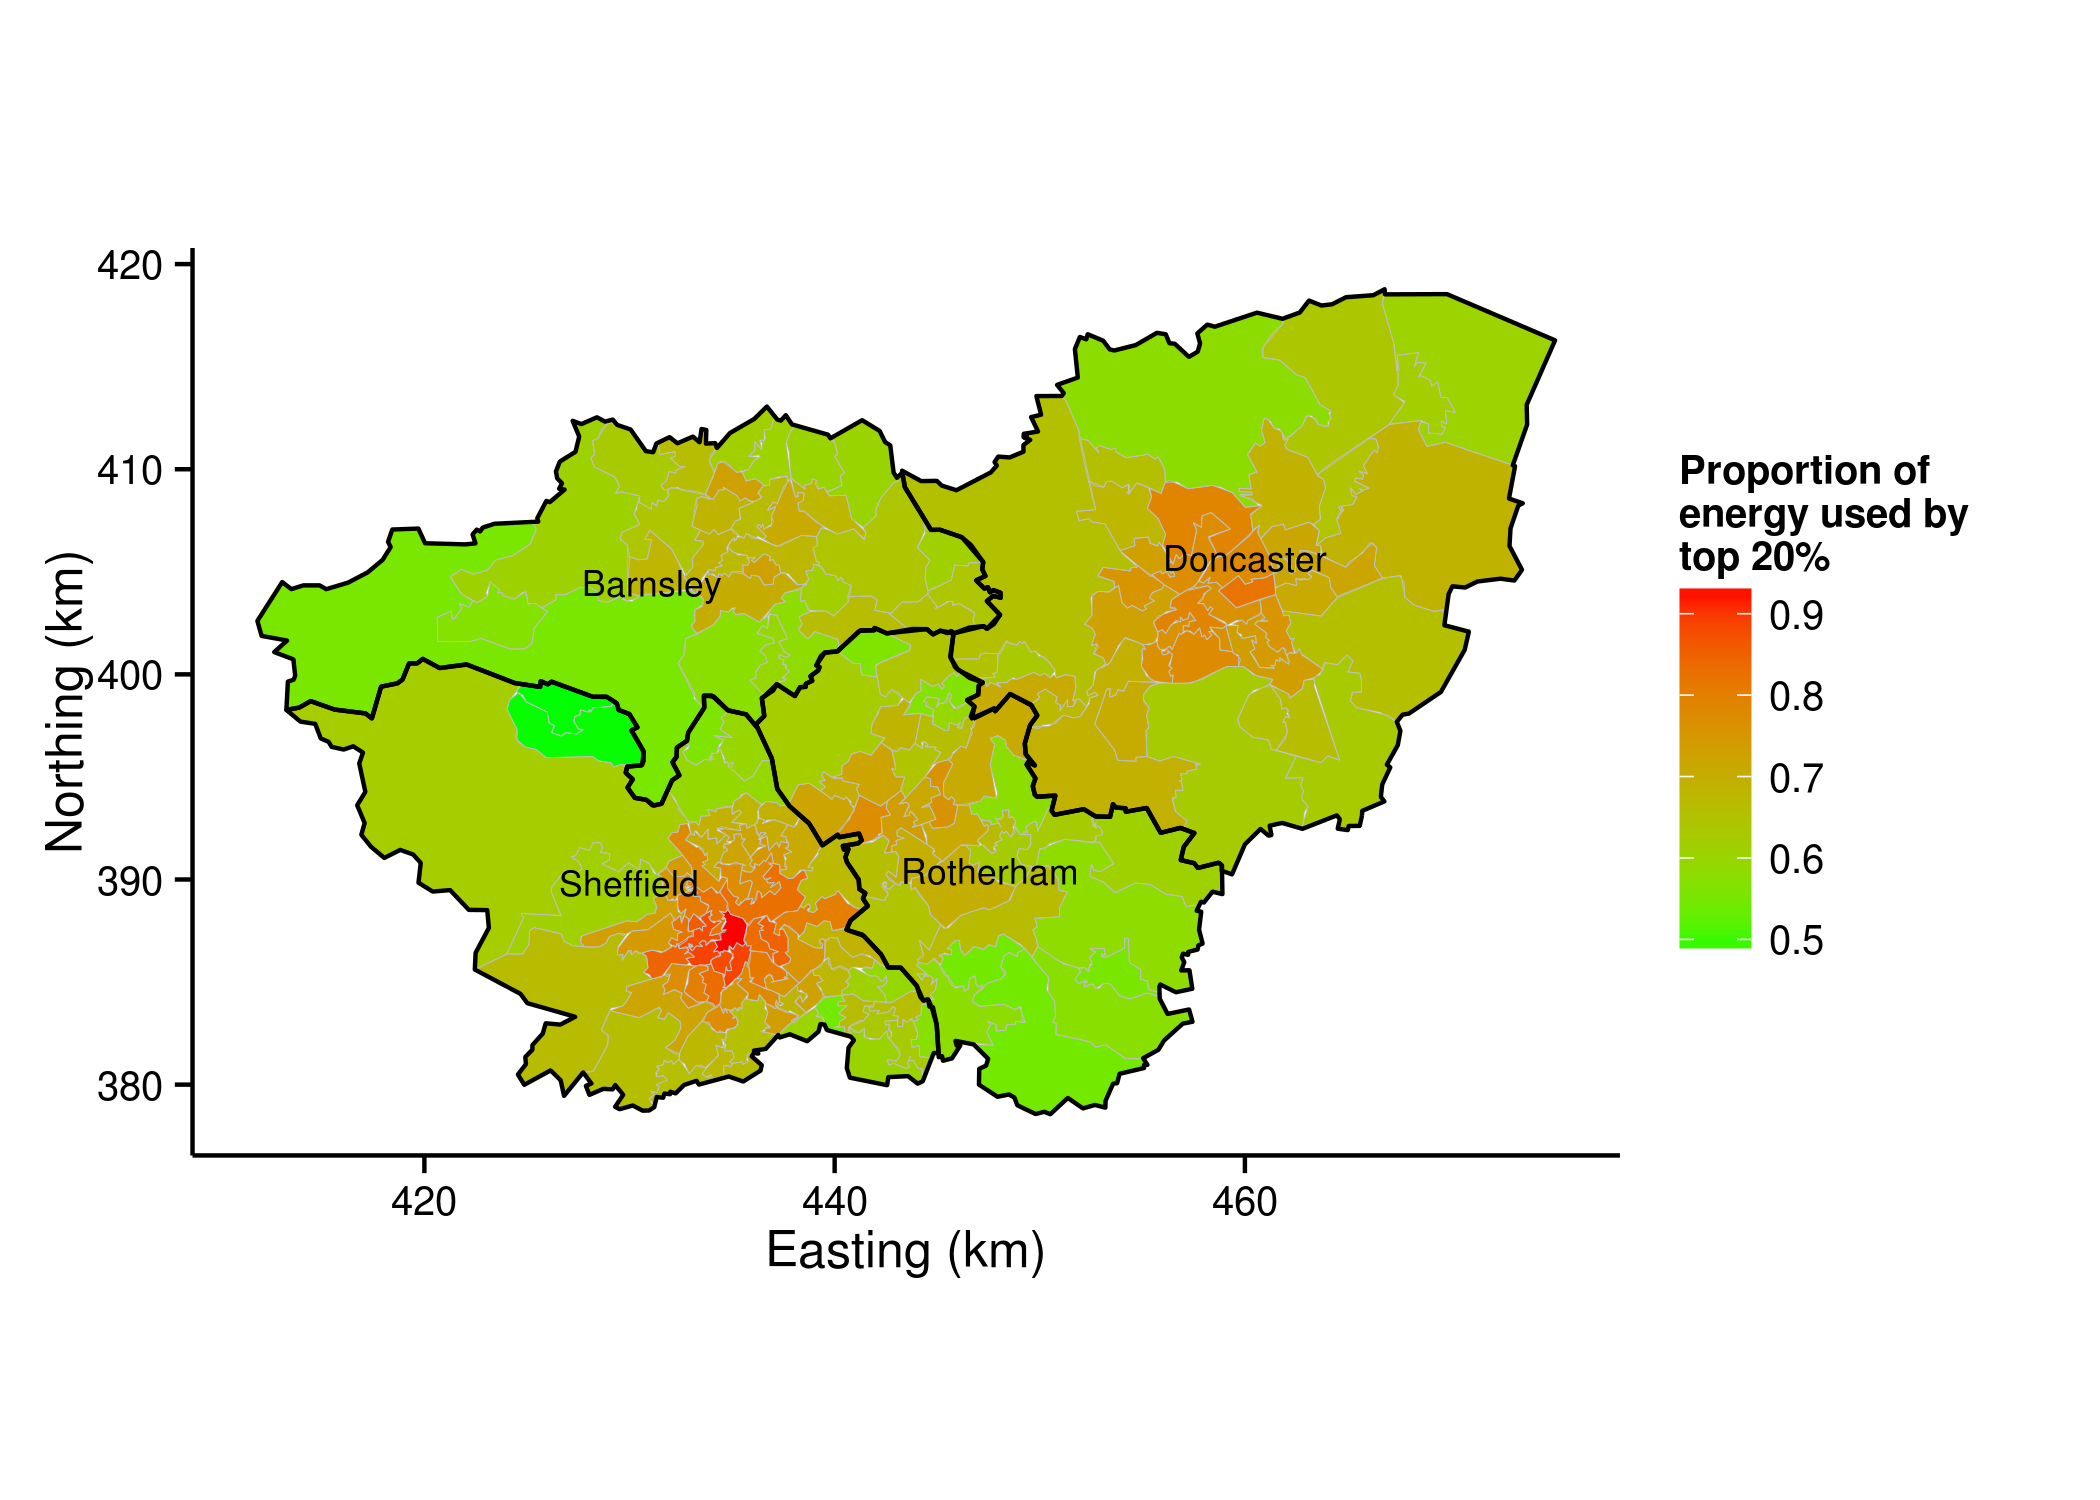
\includegraphics[width=14cm]{prop20}  \end{center}
  \caption[Proportion of energy used for commuting by the top 20\%]
  {Proportion of energy used for commuting by the top 20\% of commuters.}
 \label{fineq20}
\end{figure}

\begin{figure}[htbp]
\begin{center}
    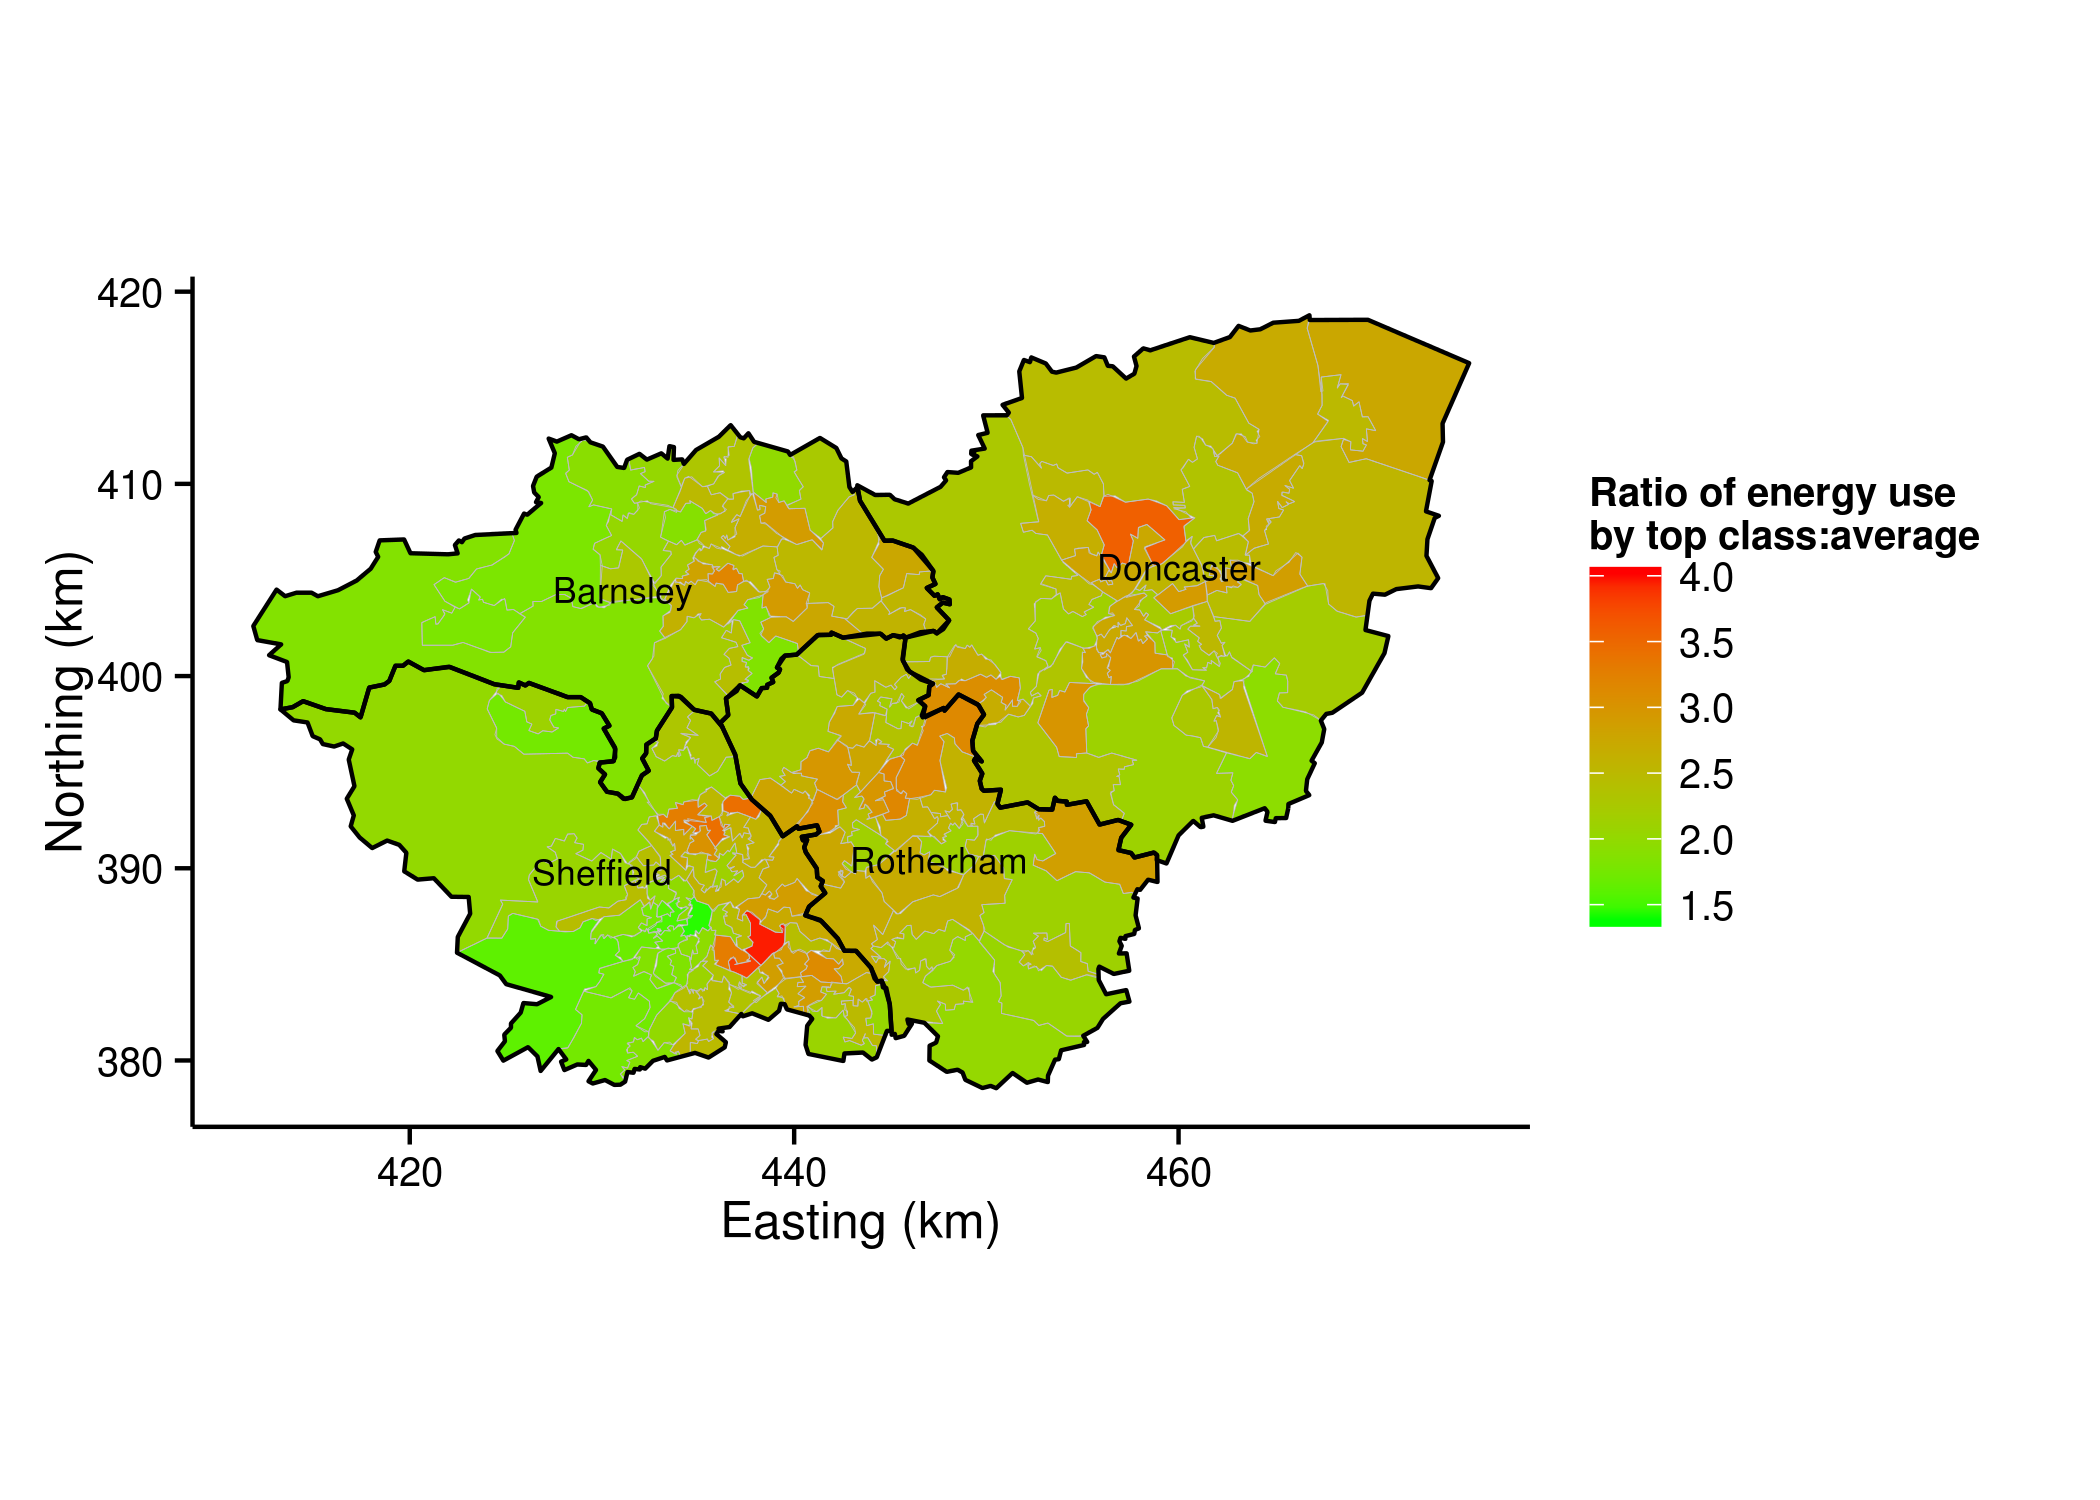
\includegraphics[width=14cm]{topprop}  \end{center}
  \caption[Relative energy use by top social classes]
  {Relative energy use by top social classes in South Yorkshire.}
 \label{ftopprop}
\end{figure}

\section{Changes over time}
As seen in the gradual improvements in car fleet efficiencies reported in
\cref{Chapter5}, the rate of energy use in transport systems is in constant
flux due to changing technologies. While efficiency improvements tend
to be gradual and predictable (due to regulation, and the long lead times
in car model development), human behaviour is not. It can respond rapidly
and unexpectedly to external factors, such as the oil price
spike of 2008 \citep{Sexton2011} and can be shifted
by emergency measures such as food rationing, conscription and
enforced agricultural and mine labour policies in World War II.

More mundane shifts in behaviour have affected the energy costs of commuting
in recent years, including the rise of `telecommuting', `flexi-time', increased
labour mobility and the tendency of people to start families far from their
home. Over the last 300 years the most important change
in commuting behaviour has been its emergence as a common activity:
before the industrial revolution and
the emergence of centralised factories,
many people worked in `cottage industries' at home. A common arrangement in rural
areas in the
1800s, for example, was for the men to work long hours (50 + per week) on
neighbouring farmland, while women worked at home \citep{groves1949sharpen}.
From the historical literature
it is clear that the energy costs of transport to work
before the industrial revolution were very low indeed, consisting primarily of
people walking a mile or two to work and a relatively small number of
horse-drawn carriages for the wealthy whilst the majority of
of the population worked from or very near to home.

To gain insight into commuting energy use before the advent of
large official databases on work and travel to work
behaviour, anecdotal and archival evidence must be relied upon. Over the
past 100 years there has been a trend towards official
data collection, analysis, storage and dissemination. In the last 50 years,
this tendency has been greatly accelerated and automated by the `digital
revolution', as mentioned in \cref{Chapter3}.
Still, before 1971 (when travel to work is first made available as a
Census variable) the best source of commuting data that could be
found was from a retrospective survey of elderly people, asked about their
past travel to work habits. %!!!
The longest yet in some ways simplest data available on commuting


\section{A comparison of commuter energy use in England and the Netherlands}
\label{sinternational}
In order to demonstrate that the methods can be used internationally,
this section provides a short case study, comparing the energy costs
of home-work travel in England and the Netherlands. These countries
were chosen for the following reasons:
\begin{itemize}
 \item Geographically aggregated data could be found for both.
 \item There are reasons to expect the Netherlands to have commuting energy costs
 substantially different from those in England. The working hypothesis we
 set-out to test was that the Netherlands would have lower energy costs, primarily
 due to the high uptake of cycling, for which the nation is famous.
 \item The countries are similar `on paper', in terms of population density,
 GDP per capita and culture.
\end{itemize}
The final point is illustrated in \cref{tcompare}, which shows the extent to
which England and the Netherlands are similar according to a handful of basic
measures. One major difference between the two countries is in terms of
income inequality, with England being substantially more unequal.
If only \cref{tcompare} were considered, we would assume that the energy
costs of commuting would be roughly the same in the two countries. However,
a couple of factors led to the hypothesis that commuting in the Netherlands
would be less energy-intensive: its relative size (42,000 km$^2$ vs 130,000 km$^2$
for England) and its famously high rate of cycling, which account for
27\% of trips nationwide and above 50\% of trips in many cities \citep{Pucher2008}.

\begin{table}[htbp]
\caption{Comparison of basic national attributes in England and the Netherlands}
\begin{center}
\begin{tabular}{llrl}
\toprule
Attribute & England & \multicolumn{1}{l}{Netherlands } & Units \\
\midrule
Population density & \multicolumn{1}{r}{407} & 406 & ppl/km2 \\
GDP & \multicolumn{1}{r}{50000} & 46000 & \$/capita \\
Income inequality & 41 (UK) & 31 & Gini Index \\
Wellbeing & 0.875 (UK) & 0.921 & UN HDI \\
\bottomrule
\end{tabular}\end{center}
\label{tcompare}
\end{table}

The input dataset for the Netherlands came in a different form from
that of England. The English data, downloaded from the Census,
provided 88 key columns from which energy values were generated:
8 distance bins for 11 modes of transport. Based on average route distances
estimated for each of the 8 Euclidean distance bins for the 8 modes whose
energy costs are described in \cref{sfinal}, the energy costs per one-way
trip were calculated for each cell in all of the 88 columns. The values in
each of the cells of the English data are people counts, so we know how many
people travelled by each mode in each distance category.
The Dutch dataset, on the other hand, provided proportions, average distances
and average times for 8 modes of transport in a wide format (\cref{tdutch}).
The first challenge upon receiving this dataset was to understand the
table's structure and translate the column headings into English.
Another issue was finding Geographical data for Dutch provinces and their
populations (this allowed for the energy costs per province to be weighted,
to provide an accurate estimate of average energy costs per commuter trips
nationwide). This data was provided by the open-data initiative
Natural Earth.\footnote{\href{http://www.naturalearthdata.com/}
{http://www.naturalearthdata.com/}
}
Finally, the commuting dataset was matched to the geographical shapefile
data in %!!! add reference of the files where this is done.
R.\footnote{Initially
this stage was problematic, as was discovered when the regions were
plotted with their name codes highlighted: the names were not associated
with the correct geographical areas. The R code used was reviewed at
each stage and it was discovered that the error was introduced through
the ``merge()'' function, which allocated the tabular data to the
geographical data by matching the zone codes. It was found that the
default (silent) default argument of ``merge()''~is ``sort=TRUE'' .
This meant that the function was re-ordering the geographical data
alphabetically. Adding ``sort=F'' ~into the command solved the problem.
}
Despite these data preparation issues, the Dutch dataset
was in fact easier to convert into average energy costs per trip than
the UK data, as it was simply the product of mode efficiency ($Ef$), average
route distance ($dR$) and modal split ($p$) for each mode:
\begin{equation}
 Etrp = \sum_m p_m \times Ef_m \times \bar{dR}_m
\end{equation}
This formula was applied to Dutch regional data, and aggregate energy costs
were calculated for England using the method described in \cref{snational}.
The results, illustrated in \cref{fdutchen}, came as a surprise:
energy use for commuting is \emph{higher} in the Netherlands, which is relatively
small, bicycle-friendly and has a low GDP, than in England. The difference
is not as great as that represented in \cref{fdutchen} (a 14\% difference,
when energy use per trip is averaged across all zones), because the zones
are not of equal population or size. When commuter energy costs are
weighted by population, the overall average energy cost per commuter trip
is still higher in the Netherlands, but less so --- 8\%:
37.5 MJ/trip in the Netherlands against 34.5 MJ/trip in England.

\begin{figure}
\centering{
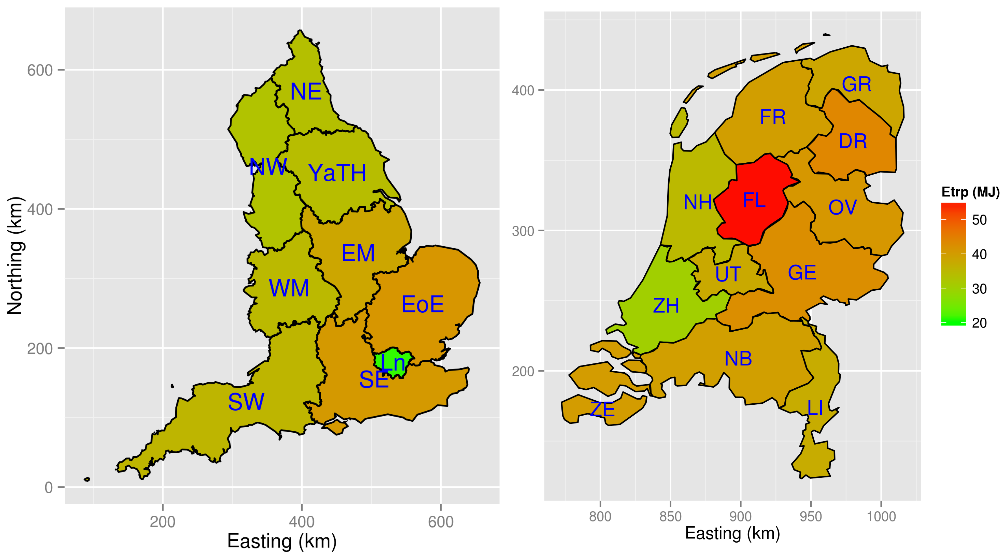
\includegraphics[width=12cm]{dutchen}
\label{fdutchen}
}
 \caption[Comparison of commuter energy use in England and the Netherlands]
 {Comparison of commuter energy use in England and the Netherlands}
\end{figure}

To explore this non-intuitive result, the first stage was to look at the modal
split of commuting in England and the Netherlands (\cref{fdutchmode}).
As expected, Dutch commuters are far more likely to travel to work by bicycle.
However, they are also less likely to travel to work by walking, as a car
passenger or by metro (due primarily to the London Underground) --- all low-energy
modes --- than UK commuters. The proportion of people travelling by car,
the most energy-intensive personal travel mode, is  only slightly lower in the
Netherlands (57\%) than in England (60\%) despite the 27\% of trips made by
bicycle. Modal split cannot account for
unexpectedly high Dutch commuter energy costs.

\begin{figure}
\centering{
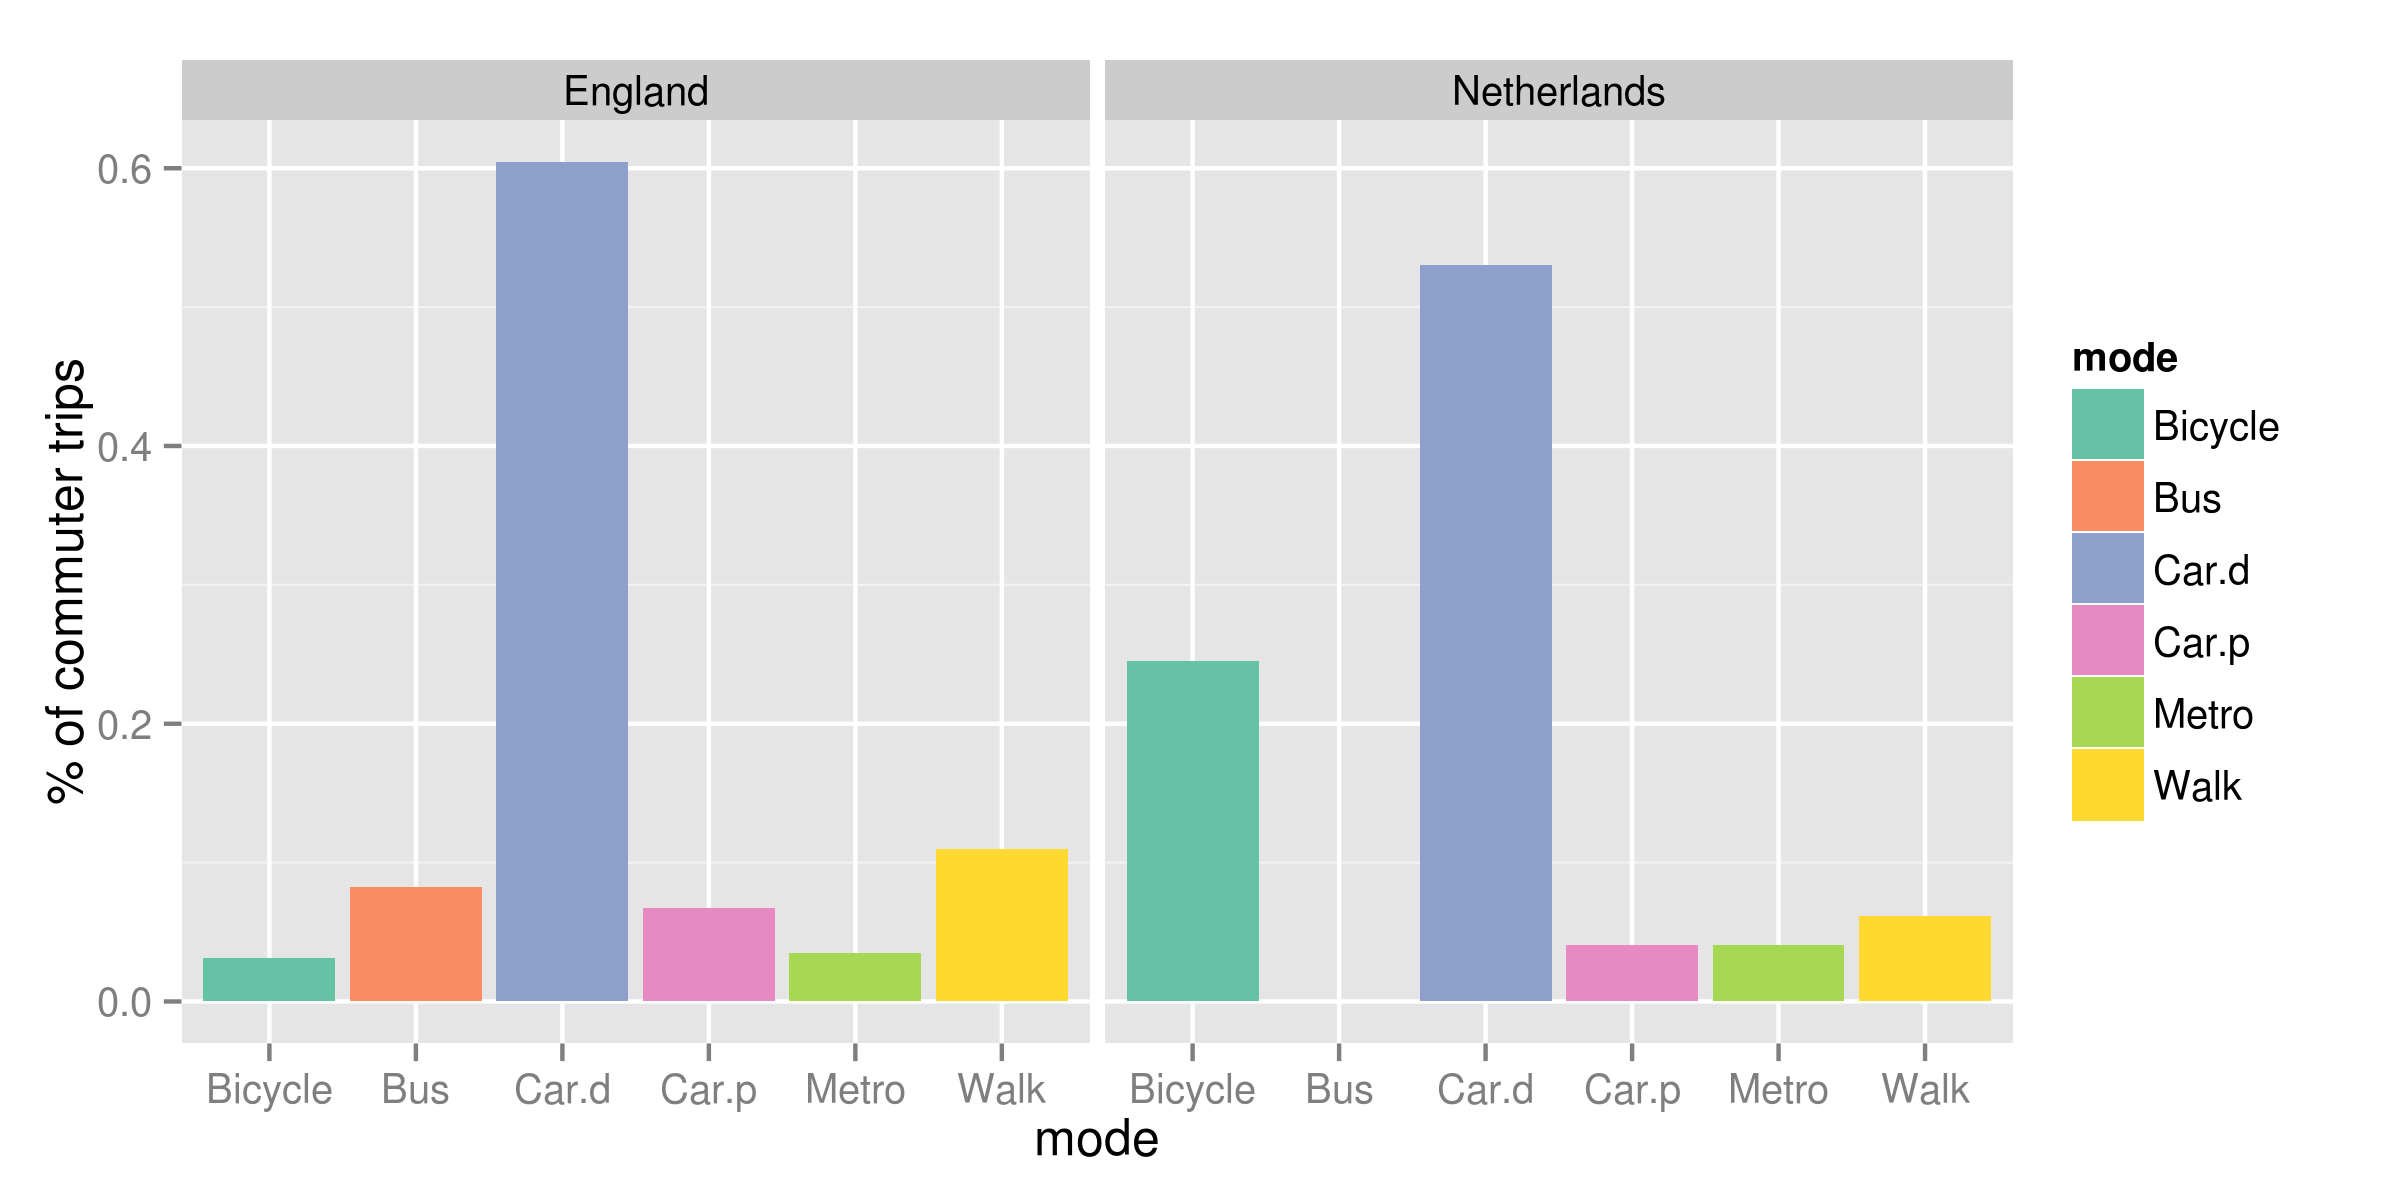
\includegraphics[width=12cm]{envsnl-modesplits}}
 \caption[Modal split of commuter trips in England and the Netherlands]
 {Modal split of commuter trips in England and the
Netherlands}\label{fdutchmode}
\end{figure}

The next variable explored was distance. The average Dutch
commute for the major forms of transport %%% The overall average is 17.6km!!!
is 1 km further than the English average at 15.5 km, from the data.
This may seem like a small amount, yet it is almost 7\% further, accounting for
most of the variability in energy use. When we
break this figure down by mode, as in \cref{favdistnl}, it becomes clear that
car trips are the reason for the increased distance of travel to work
in the Netherlands: all other modes are associated with shorter trip distances,
whereas the average commuter trip by car, the most energy intensive transport
mode, is \emph{30\%} further than in England (24.6 km in
the Netherlands, compared with 18.7 km). It therefore seems that
the prevalence of one particular trip type --- long car trips --- explains why
commuter energy use in the Netherlands is greater, per person, than in the UK.

% !!! spatial distribution???

\begin{figure}
\centering{
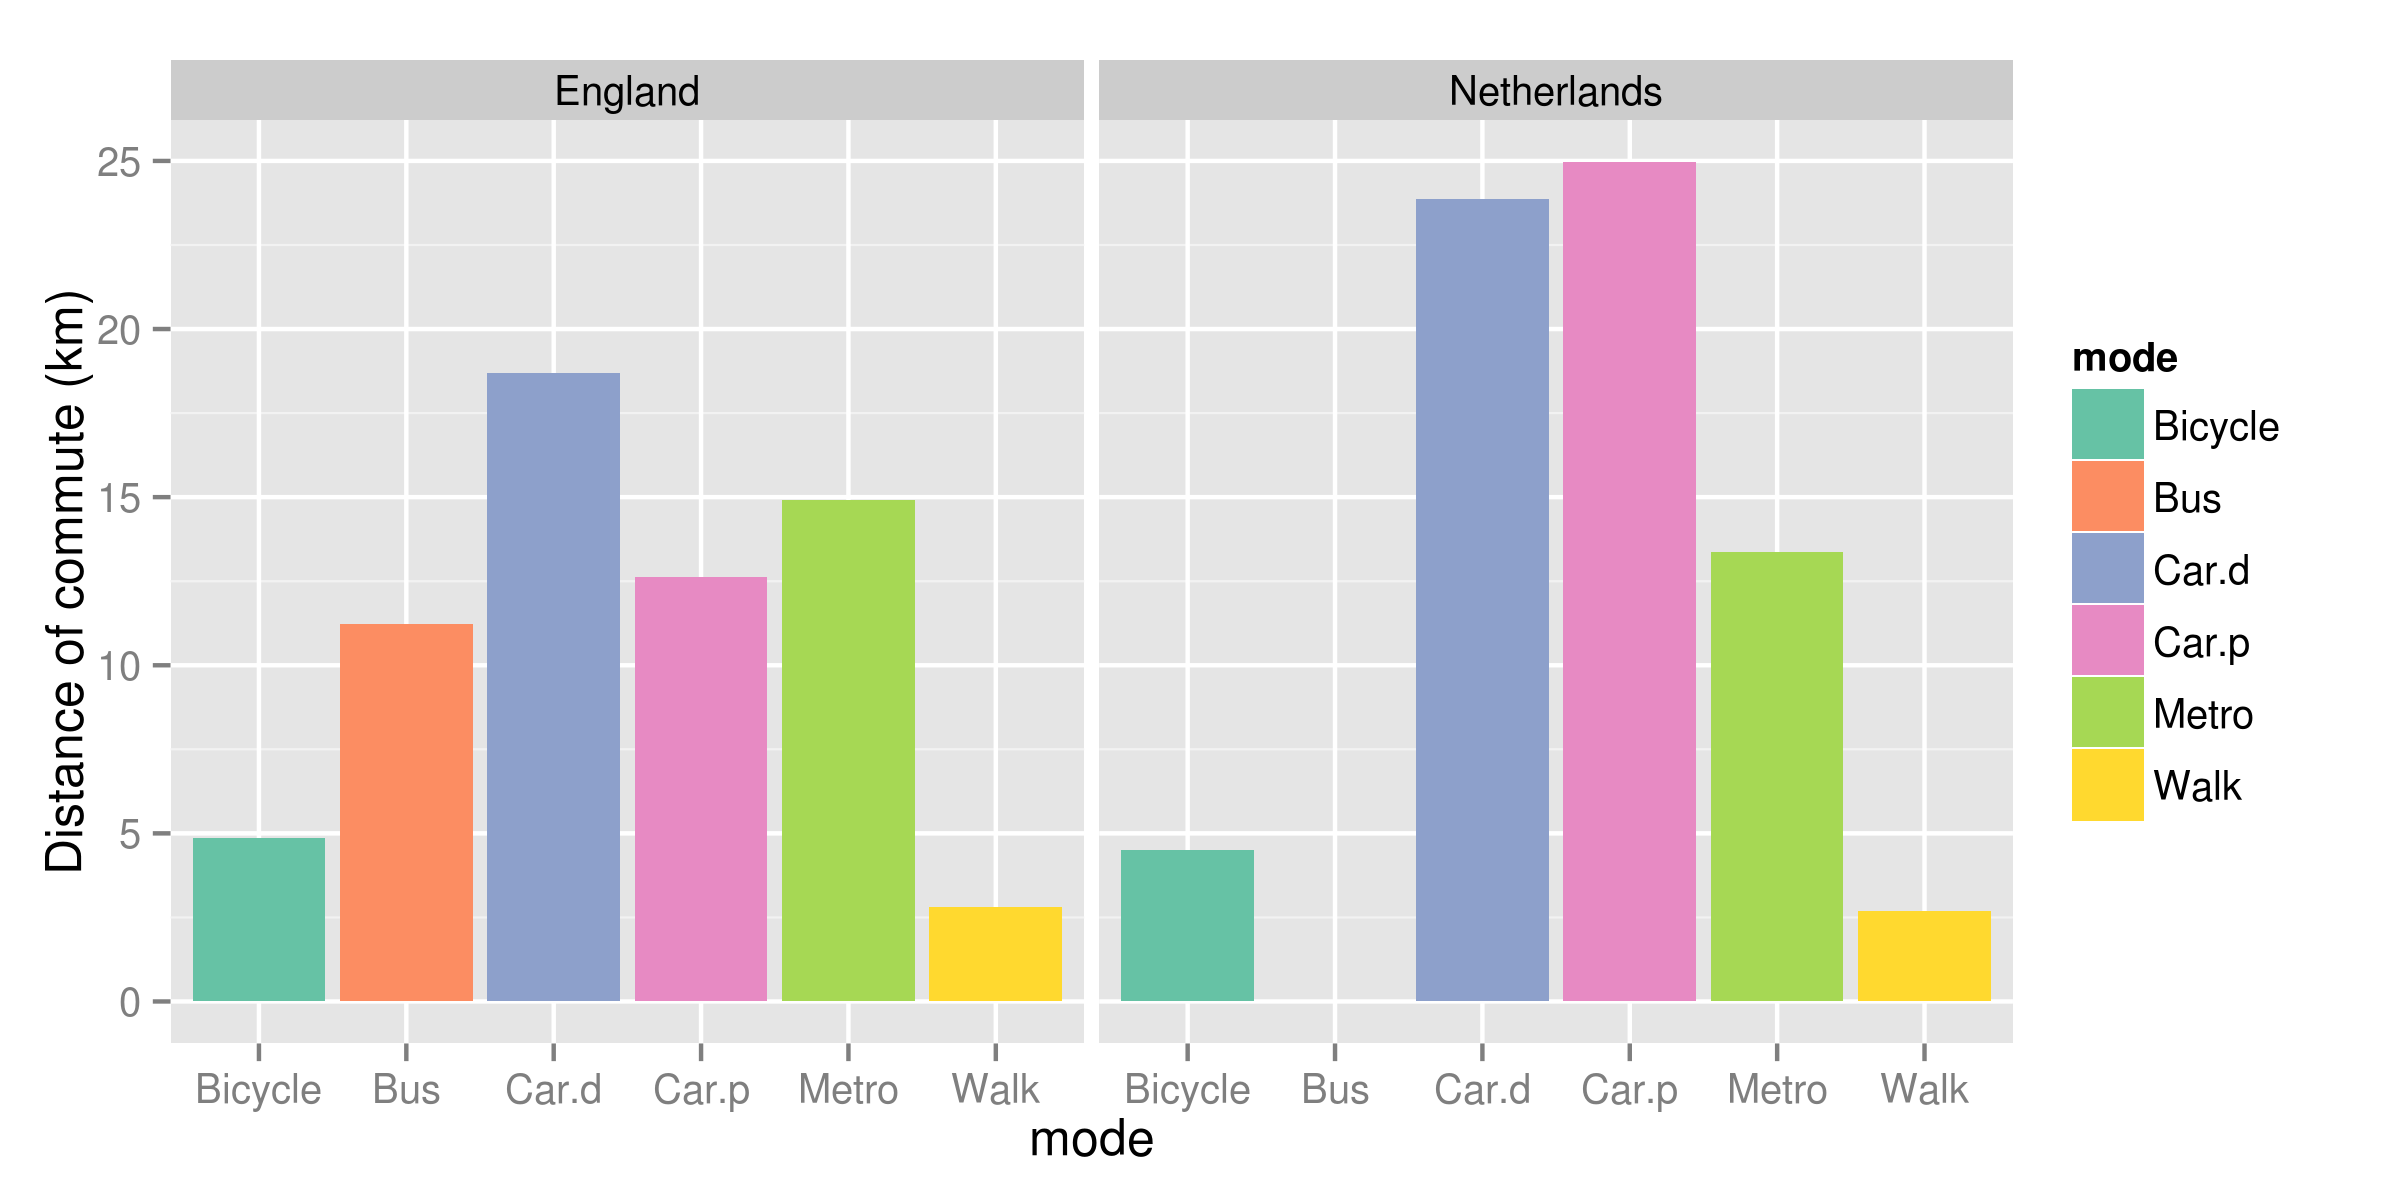
\includegraphics[width=12cm]{avdist-nl-en}}
 \caption[Distance of commuting by mode, England and the Netherlands]
 {Average distance of commuter trip by mode in England and the
Netherlands}\label{favdistnl}
\end{figure}

\begin{table}[htbp]
\caption[Sample of the raw Dutch commuting data]
{Sample of the first 4 columns of the raw Dutch commuting data. A further 54
columns on the proportions travelling by and average time and distances of
trips by 9 modes of transport are not shown.}
\centering{\begin{tabular}{lrrr}
\toprule
Perioden & 2010 & 2010 & 2010 \\
Vervoerwijzen & \multicolumn{1}{l}{Totaal} & \multicolumn{1}{l}{Auto (bestuurder)} & \multicolumn{1}{l}{Auto (passagier)} \\
Regio's & \multicolumn{1}{l}{aantal} & \multicolumn{1}{l}{aantal} & \multicolumn{1}{l}{aantal} \\
\midrule
Nederland & 0.48 & 0.25 & 0.03 \\
Groningen (PV) & 0.44 & 0.22 & 0.03 \\
Friesland (PV) & 0.45 & 0.24 & 0.02 \\
Drenthe (PV) & 0.46 & 0.29 & 0.03 \\
Overijssel (PV) & 0.48 & 0.26 & 0.03 \\
Flevoland (PV) & 0.51 & 0.28 & 0.04 \\
Gelderland (PV) & 0.47 & 0.26 & 0.03 \\
Utrecht (PV) & 0.5 & 0.23 & 0.03 \\
Noord-Holland (PV) & 0.48 & 0.22 & 0.03 \\
Zuid-Holland (PV) & 0.49 & 0.23 & 0.03 \\
Zeeland (PV) & 0.47 & 0.27 & 0.03 \\
Noord-Brabant (PV) & 0.47 & 0.28 & 0.04 \\
Limburg (PV) & 0.46 & 0.28 & 0.03 \\
\bottomrule
\end{tabular}}
\label{tdutch}
\end{table}

Regarding the spatial distribution of energy-intensive commuting,
there is no clear pattern at this coarse level of geographical aggregation.
A pattern does emerge when we plot energy use against
population density (\cref{fepdensnl}), which shows a strong negative correlation
(r = -0.7, p $<$ 0.001) between the two variables. The two clear outliers in
terms of energy use are London (20.8 MJ/trip) and Flevoland (54.8 MJ/trip),
which are the also on opposite ends of the population density scale.
\Cref{fepdensnl} is also useful as it shows there is a large amount of
overlap in commuter energy between the two countries, even at this high
level of geographical aggregation. Three English regions
(the South East, East of England and the East Midlands) have average
commuter energy costs above the Dutch national average; interestingly
each of these zones is quite wealthy, with strong links to London
(implying commuting to London may be a cause of high energy use here).
The only Dutch province with average commuter energy costs below the
English average is Zuid (meaning South) Holland. This area has a very high
population density and includes large cities including the Hague and
Rotterdam.

\begin{figure}
 \centering{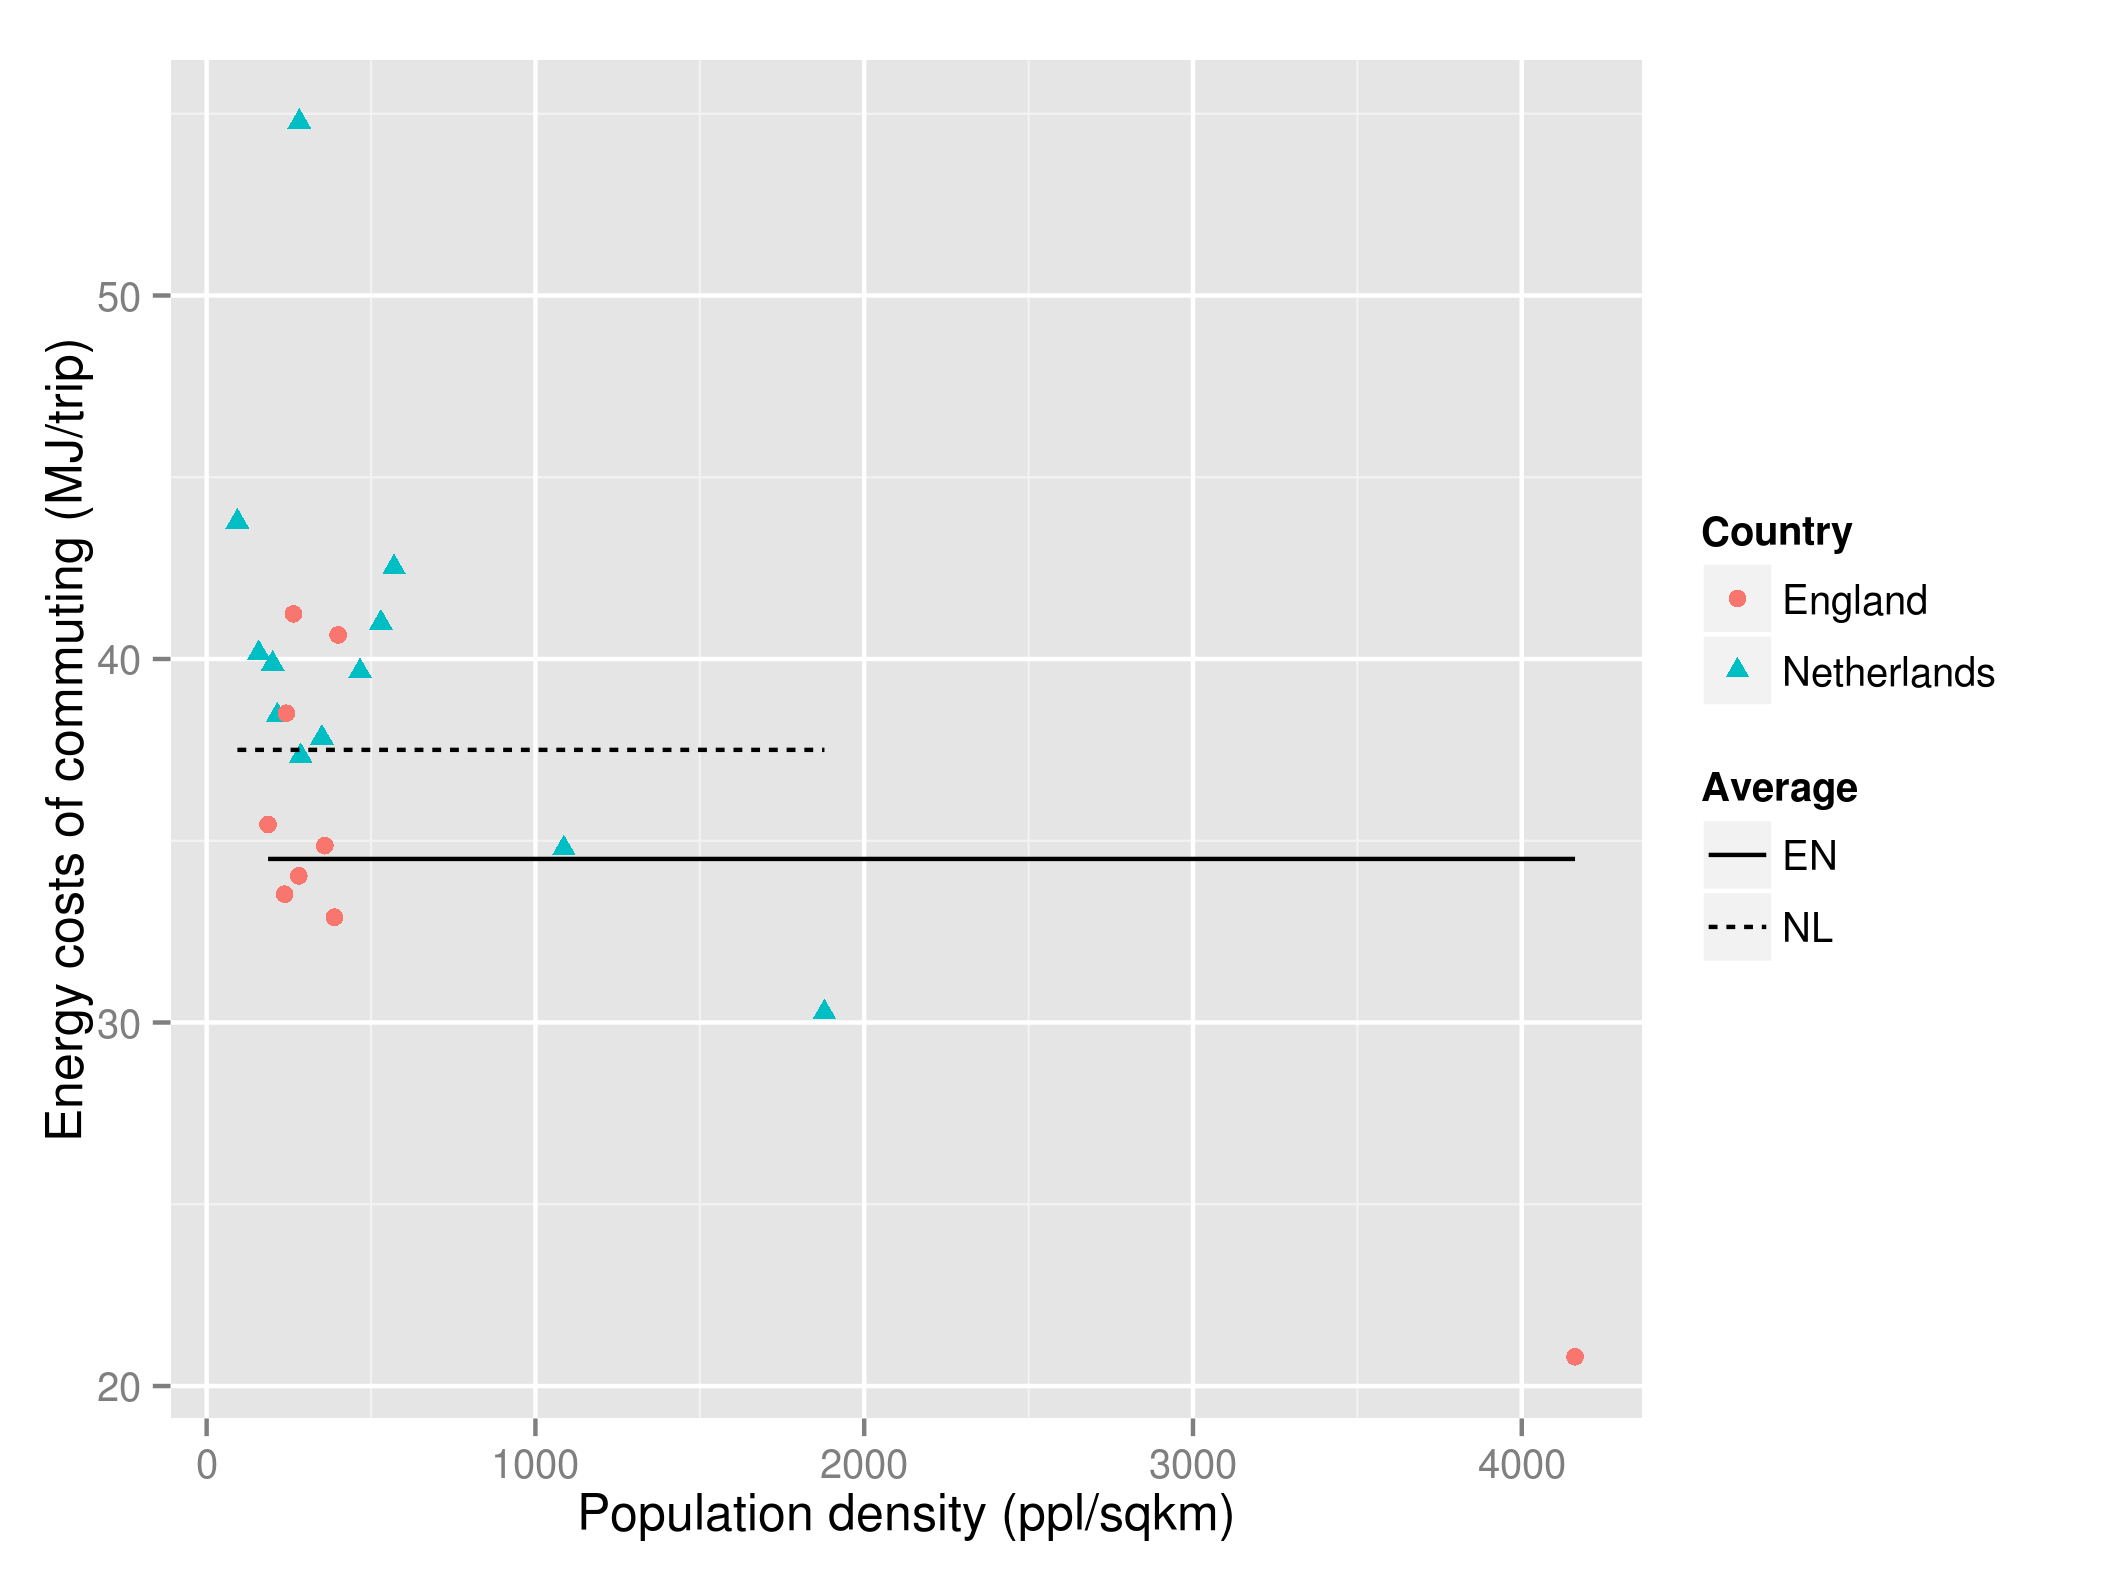
\includegraphics[width=12cm]{epdensnl}}
 \caption[Population density against commuter energy use]
 {Population density against commuter energy use, in Netherlands and England}
 \label{fepdensnl}
\end{figure}

\subsection{Data inconsistencies and caveats}
A problem with the preceding national level comparison is that the
data come from different years, 2001 and 2010 for England and the Netherlands
respectively. One could argue that this is not an issue
from the perspective of demonstrating the international applicability of the
methods. However, it is a major problem if we aim to use the empirical results,
for example to argue that a focus on modal split alone may not be  effective at
increasing the sustainability of personal travel, if distance is not considered
as well. %!!! add a link here
The claim that energy use per commute is greater in the Netherlands is
higher than in England is also an interesting result in itself and merits
evaluation of the quality of the data and analysis that led to this result.

\Cref{fcommuterdistime} shows that the length of commuter trips in Great
Britain (including Wales and Scotland) has remained steady over
time. It increased by only 5\% between 1995/1997 and 2009 and only by
1\% between 2002 (the closest data point to 2001) and 2009. In addition,
\cref{fmode-time-dft2011} demonstrates that the modal split of commuter trips
has also been relatively steady, with slight declines in car use suggesting that
energy use may have even declined. 

\begin{figure}
 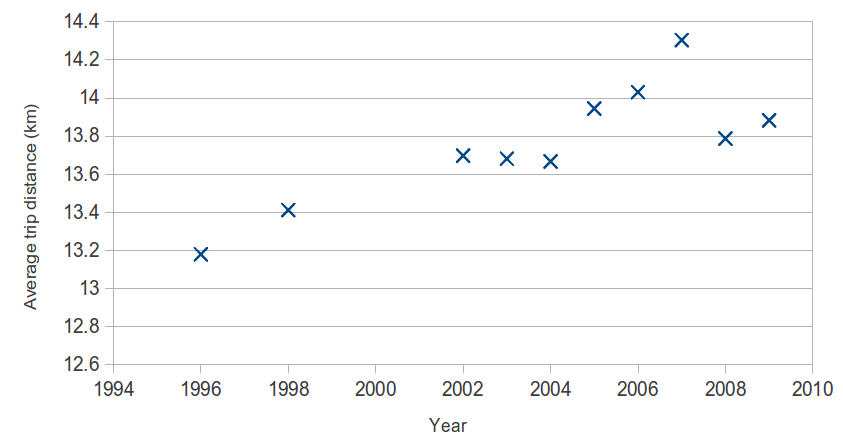
\includegraphics[width=12cm]{commuter-trip-dis-time}
 \caption[Average commuter trip distance over time in Great Britain]
 {Average commuter trip distance over time in Great Britain. Data from
 \citet[table 9]{DfT2011-commuting}, n $>$ 15,000 for every year.} \label{fcommuterdistime}
\end{figure}

\begin{figure}
 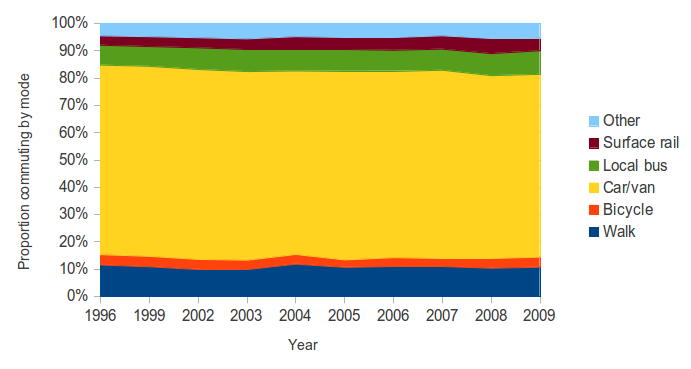
\includegraphics[width=12cm]{mode-time-dft2011}
 \caption[Modal split of commuter trips, Great Britain 1995 - 2009]
 {Modal split of commuter trips, Great Britain 1995 - 2009. Data from
 \citet[table 9]{DfT2011-commuting}, n $>$ 15,000 for every year.} \label{fmode-time-dft2011}
\end{figure}

Another issue is data quality. While both datasets
are from official sources, the Dutch data is far let detailed and provides
only two significant figures for the proportions of people travelling by each
mode (e.g. 0.01). Thus, error up to 0.5\% in these figures is possible.
Further, average distances were not provided for all modes of transport in all
areas, in which case the mode's average figure for the areas that were reported
were used to fill-in the gap. Finally, the figures for the proportion of people
travelling by train seemed very low, given that the Netherlands has an
advanced rail network. As outlined in \cref{Chapter4}, %!!! really???
there are also issues with the UK dataset. The translation of
Euclidean distance
categories into average route distances is a particularly risky
activity and may introduce error in excess of the difference between
Dutch and English average commuter trip energy costs reported above.

In light of these caveats, more robust data is needed to resolve the
enigma of the Netherlands'...'

% \section{Changes in energy use over time} \label{stime}
% 





% \section{Explaining high and low energy use} \label{sexplanation} %!!! re-add
% \index{decomposition framework}
% Regardless of technology and the various complicating factors discussed
% in \cref{svariable}, the primary determinants of the energy costs of
% personal transport are mode and distance. Focussing simply on one or the other
% (as other authors have done) omits a substantial part of the picture because it
% is the combination of an energy intensive mode and an energy intensive trip that
% leads to high energy costs. In England as a whole, the most energy intensive
% form of transport (single occupancy cars) is the most common form of transport
% to work for all but the shortest trips \cref{fengmodedis}.

\begin{figure}[htbp]
    \centering{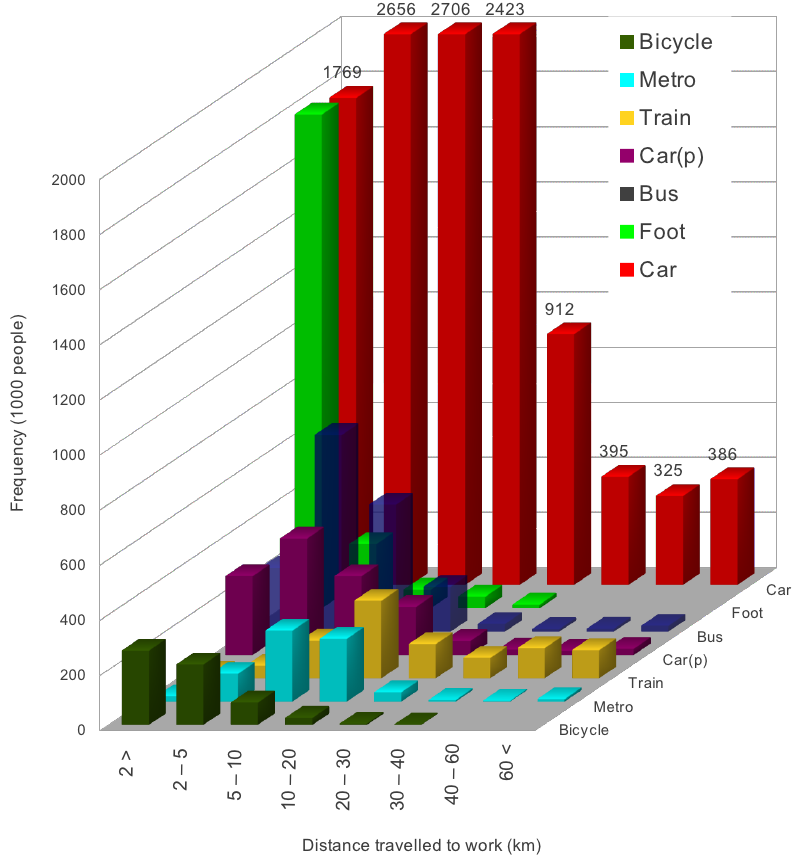
\includegraphics[width=12cm]{England-ttw-mode-distances}}
  \caption[Mode and distance categories of commute in England]
  {Mode and distance categories of commuter trips in England, 2001}
  \label{fengmodedis}
\end{figure} %!!! re-add? (hopefully!)


% The aggregate estimate of energy use is interesting in itself, allowing
% commuting energy used to be placed in context of other phenomena.
% % It should be clear that commuting is more important than many other
% % ``energy issues'' such as the efficiency of lights and solar panels,
% % which have received relatively more attention from an energy perspective from
% % policy makers and academicis. !!! put commuter energy use in perspective - fig
% However, one of the aims (A1.2, \cref{s:aims}) was also to explain why energy
% use in transport to work is as it is. As illustrated in previous literature
% \cref{Chapter2},
% many factors contribute to the total energy use in transport systems.
% To recap, these include number, distance and frequency of trips, occupancy,
% mode, fleet efficiencies, infrastructure impacts and behavioural factors such
% as driving style. %!!! refs.
% 
% This section will formalise these considerations using a framework: the
% decomposition framework \citep{}. In terms of total energy use in the economy,
% three main factors (activity, structural and energy intensity effects)
% can be modelled to explain and project growing or declining energy use
% \citep{farla2000physical}.
% This framework can be applied to the decomposition of energy use in, as
% illustrated in \cref{f:components}. Starting with decomposition by mode, the
% formulae to describe each element of the decomposition analysis are formalised
% in equations \ref{e:component1} to \ref{e:componentn}.
% 
% \begin{equation}
%  Etot = {\displaystyle \sum^m_{m=1}
% N_{trips,m} \times \overline{d}_{R,m} \times \overline{E}_{F,m}}
% \end{equation}  


\section{Uncertainties and complications} \label{suncertainties}

``correctness is usually expensive, and high correctness is often
\emph{disproportionately} more expensive'' \citep[p.~153]{janert2010data}.

% !!! Links with section in ch.4.

% \subsection{The relevance of flow data for the energy costs of travel to work}
% The route taken by a given vehicle can have a large impact on its energy use.
% This can be illustrated by considering cases of bus travel, on various
% locations of the energy efficiency spectrum:
% \begin{itemize}
%  \item dhf
% 
% \end{itemize}
% 
% On one hand,  extreme example could be the
% comparative efficiency per person of an old London bus carrying 20 people
% through clogged streets c
